\begin{enumerate}[label=\thechapter.\arabic*,ref=\thechapter.\theenumi]

\item The number of zeroes of the polynomial $P(s) = s^3+2s^2+5s+80$ in the right side of the plane?\hfill(GATE IN 2023) \\

\solution
\iffalse
\let\negmedspace\undefined
\let\negthickspace\undefined
\documentclass[journal,12pt,twocolumn]{IEEEtran}
\usepackage{cite}
\usepackage{amsmath,amssymb,amsfonts,amsthm}
\usepackage{algorithmic}
\usepackage{graphicx}
\usepackage{textcomp}
\usepackage{xcolor}
\usepackage{txfonts}
\usepackage{listings}
\usepackage{enumitem}
\usepackage{mathtools}
\usepackage{gensymb}
\usepackage{comment}
\usepackage[breaklinks=true]{adjustbox}
\usepackage{tkz-euclide} 
\usepackage{listings}
\usepackage{gvv}                                        
\def\inputGnumericTable{}                                 
\usepackage[latin1]{inputenc}                                
\usepackage{color}                                            
\usepackage{array}                                            
\usepackage{longtable}                                       
\usepackage{calc}                                             
\usepackage{multirow}                                         
\usepackage{hhline}                                           
\usepackage{ifthen}                                           
\usepackage{lscape}

\newtheorem{theorem}{Theorem}[section]
\newtheorem{problem}{Problem}
\newtheorem{proposition}{Proposition}[section]
\newtheorem{lemma}{Lemma}[section]
\newtheorem{corollary}[theorem]{Corollary}
\newtheorem{example}{Example}[section]
\newtheorem{definition}[problem]{Definition}
\newcommand{\BEQA}{\begin{eqnarray}}
\newcommand{\EEQA}{\end{eqnarray}}
\newcommand{\define}{\stackrel{\triangle}{=}}
\theoremstyle{remark}
\newtheorem{rem}{Remark}

\begin{document}
\bibliographystyle{IEEEtran}

\vspace{3cm}

\title{}
\author{EE23BTECH11024 - G.Karthik Yadav$^{*}$
}
\maketitle
\newpage
\bigskip

\section*{GATE 2023 EC 41}
\noindent 1. \hspace{2pt} A Closed loop systen is shown in the figure where $k>0$ and $\alpha>0$ .\\
The Steady State error due to a ramp input $\brak{R\brak{s} = \alpha s^{-2}}$ is given by \hfill{(GATE 2023 EC 41)}

\begin{figure}[ht]
\centering
    \includegraphics[width=1.0\linewidth]{2023/EC/41/figs/question.png}
    \label{fig: 23.EC.41.24.1}
\end{figure}

\begin{enumerate}
\item $\frac{2\alpha}{k}$
\item $\frac{\alpha}{k}$
\item $\frac{\alpha}{2k}$
\item $\frac{\alpha}{4k}$
\end{enumerate}

\solution\\
\fi
\begin{table}[ht]
\setlength{\arrayrulewidth}{0.3mm}
\setlength{\tabcolsep}{15pt}
\renewcommand{\arraystretch}{1.5}



\begin{tabular}{ |p{1cm}|p{3cm}|p{1cm}| }
\hline
Symbol & Parameters & Value\\
\hline
$R\brak{s}$ & Laplace transform Ramp input signal r\brak{t} &  $\alpha s^{-2}$\\
\hline
$G\brak{s}$ & Open Loop transfer function &  $ \frac{Y\brak{s}}{E\brak{s}} = \frac{k}{s\brak{s+2}}$\\
\hline
$Y\brak{s}$ & Laplace transform of the output signal y\brak{t}  &  ? \\
\hline
$E\brak{s}$ & Laplace transform of the error signal e\brak{t} & R\brak{s} - Y\brak{s}\\
\hline
$E\brak{s}$ & Laplace transform of the error signal e\brak{t} & R\brak{s} - Y\brak{s}\\   
\hline
$e_s$ & Steady State Error &  ? \\
\hline
%$x(l)$ & Last($l^{th}$) term of series & 350\\
%$x(0)$ & Starting ($0^{th}$) term of series & 17 %\\
%\hline
%d & Common difference of AP & 9\\
%\hline
\end{tabular}
\caption{Parameters}






\end{table}
\bigskip
from table  Open loop transfer function $G\brak{s}$\\
\begin{align}
	G\brak{s} &= \frac{Y\brak{s}}{E\brak{s}} \label{24.2023.EC.41.1} \\
        &= \frac{Y\brak{s}}{R\brak{s} - Y\brak{s}} \\
        Y\brak{s} &= \frac{R\brak{s}G\brak{s}}{1 + G\brak{s}} \label{24.2023.EC.41.2}
\end{align}

from eq \ref{24.2023.EC.41.1} and eq \eqref{24.2023.EC.41.2}

\begin{align}
        G\brak{s} &= \frac{k}{s\brak{s +2}}  \label{24.2023.EC.41.3} \\ 
        Y\brak{s} &= \frac{\alpha k s^{-2}}{k + s\brak{s+2}} \label{24.2023.EC.41.4} \\
        E\brak{s} &= R\brak{s} - Y\brak{s}  \label{24.2023.EC.41.5} \\ 
        E\brak{s} &= \frac{\alpha \brak{s+2}}{s\brak{k + s\brak{s+2}}}
\end{align}

By Taking Inverse Laplace Transform of eq \eqref{24.2023.EC.41.3} and eq\eqref{24.2023.EC.41.4}

\begin{align}
    g\brak{t} &= \frac{k\brak{1 - e^{-2t}}}{2} u\brak{t} \\
        y\brak{t} &= \alpha t u\brak{t}- \frac{2\alpha}{k}u\brak{t} \\
        \notag &+\frac{\alpha}{2k\sqrt{1-k}} \biggl(2\sqrt{1-k}e^{\sqrt{1-k}t-1}\\ 
        \notag &+ 2\sqrt{1-k}e^{-\sqrt{1-k}t-1} \\
        \notag &+ \brak{2-k}e^{\sqrt{1-k}t-1} - \brak{2-k}e^{-\sqrt{1-k}t-1} \biggr) u\brak{t}
\end{align}

\begin{align}
        e\brak{t} &= r\brak{t} - y\brak{t} \\
        &= \alpha t u\brak{t} - y\brak{t} \\
        e\brak{t} &= \frac{2\alpha}{k}u\brak{t} \\
        \notag &-\frac{\alpha}{2k\sqrt{1-k}} \biggl(2\sqrt{1-k}e^{\sqrt{1-k}t-1}\\ 
        \notag &+ 2\sqrt{1-k}e^{-\sqrt{1-k}t-1} \\
        \notag &+ \brak{2-k}e^{\sqrt{1-k}t-1} - \brak{2-k}e^{-\sqrt{1-k}t-1} \biggr) u\brak{t}
\end{align}
	

\begin{align}
    e_s &= \displaystyle\lim_{s\to 0}s E\brak{s} \\
    &= \displaystyle\lim_{s\to 0} s \frac{R\brak{s}}{1 + G\brak{s}} \\
    &= \displaystyle\lim_{s\to 0} \frac{\alpha \brak{s+2}}{s\brak{s+2} + k} \\
    e_s &= \frac{2\alpha}{k}
\end{align}



\newpage

\item The circuit shown in the figure is initially in the steady state with the switch K in open condition and $\overline{K}$ in closed condition. The switch K is closed and $\overline{K}$ is opened simultaneously at the instant $t = t_1$, where $t_1 > 0$. The minimum value of $t_1$ in milliseconds such that there is no transient in the voltage across the 100 $\mu F$ capacitor, is \rule{1cm}{0.15mm} (Round off to 2 decimal places) \hfill (GATE EE 2023)
\input{2023/EE/54/figs/ckt1.tex}\\
\solution
\iffalse
\let\negmedspace\undefined
\let\negthickspace\undefined
\documentclass[journal,12pt,twocolumn]{IEEEtran}
\usepackage{cite}
\usepackage{amsmath,amssymb,amsfonts,amsthm}
\usepackage{algorithmic}
\usepackage{graphicx}
\usepackage{textcomp}
\usepackage{xcolor}
\usepackage{txfonts}
\usepackage{listings}
\usepackage{enumitem}
\usepackage{mathtools}
\usepackage{gensymb}
\usepackage{comment}
\usepackage[breaklinks=true]{adjustbox}
\usepackage{tkz-euclide} 
\usepackage{listings}
\usepackage{gvv}                                        
\def\inputGnumericTable{}                                 
\usepackage[latin1]{inputenc}                                
\usepackage{color}                                            
\usepackage{array}                                            
\usepackage{longtable}                                       
\usepackage{calc}                                             
\usepackage{multirow}                                         
\usepackage{hhline}                                           
\usepackage{ifthen}                                           
\usepackage{lscape}

\newtheorem{theorem}{Theorem}[section]
\newtheorem{problem}{Problem}
\newtheorem{proposition}{Proposition}[section]
\newtheorem{lemma}{Lemma}[section]
\newtheorem{corollary}[theorem]{Corollary}
\newtheorem{example}{Example}[section]
\newtheorem{definition}[problem]{Definition}
\newcommand{\BEQA}{\begin{eqnarray}}
\newcommand{\EEQA}{\end{eqnarray}}
\newcommand{\define}{\stackrel{\triangle}{=}}
\theoremstyle{remark}
\newtheorem{rem}{Remark}

\begin{document}
\bibliographystyle{IEEEtran}

\vspace{3cm}

\title{}
\author{EE23BTECH11024 - G.Karthik Yadav$^{*}$
}
\maketitle
\newpage
\bigskip

\section*{GATE 2023 EC 41}
\noindent 1. \hspace{2pt} A Closed loop systen is shown in the figure where $k>0$ and $\alpha>0$ .\\
The Steady State error due to a ramp input $\brak{R\brak{s} = \alpha s^{-2}}$ is given by \hfill{(GATE 2023 EC 41)}

\begin{figure}[ht]
\centering
    \includegraphics[width=1.0\linewidth]{2023/EC/41/figs/question.png}
    \label{fig: 23.EC.41.24.1}
\end{figure}

\begin{enumerate}
\item $\frac{2\alpha}{k}$
\item $\frac{\alpha}{k}$
\item $\frac{\alpha}{2k}$
\item $\frac{\alpha}{4k}$
\end{enumerate}

\solution\\
\fi
\begin{table}[ht]
\setlength{\arrayrulewidth}{0.3mm}
\setlength{\tabcolsep}{15pt}
\renewcommand{\arraystretch}{1.5}



\begin{tabular}{ |p{1cm}|p{3cm}|p{1cm}| }
\hline
Symbol & Parameters & Value\\
\hline
$R\brak{s}$ & Laplace transform Ramp input signal r\brak{t} &  $\alpha s^{-2}$\\
\hline
$G\brak{s}$ & Open Loop transfer function &  $ \frac{Y\brak{s}}{E\brak{s}} = \frac{k}{s\brak{s+2}}$\\
\hline
$Y\brak{s}$ & Laplace transform of the output signal y\brak{t}  &  ? \\
\hline
$E\brak{s}$ & Laplace transform of the error signal e\brak{t} & R\brak{s} - Y\brak{s}\\
\hline
$E\brak{s}$ & Laplace transform of the error signal e\brak{t} & R\brak{s} - Y\brak{s}\\   
\hline
$e_s$ & Steady State Error &  ? \\
\hline
%$x(l)$ & Last($l^{th}$) term of series & 350\\
%$x(0)$ & Starting ($0^{th}$) term of series & 17 %\\
%\hline
%d & Common difference of AP & 9\\
%\hline
\end{tabular}
\caption{Parameters}






\end{table}
\bigskip
from table  Open loop transfer function $G\brak{s}$\\
\begin{align}
	G\brak{s} &= \frac{Y\brak{s}}{E\brak{s}} \label{24.2023.EC.41.1} \\
        &= \frac{Y\brak{s}}{R\brak{s} - Y\brak{s}} \\
        Y\brak{s} &= \frac{R\brak{s}G\brak{s}}{1 + G\brak{s}} \label{24.2023.EC.41.2}
\end{align}

from eq \ref{24.2023.EC.41.1} and eq \eqref{24.2023.EC.41.2}

\begin{align}
        G\brak{s} &= \frac{k}{s\brak{s +2}}  \label{24.2023.EC.41.3} \\ 
        Y\brak{s} &= \frac{\alpha k s^{-2}}{k + s\brak{s+2}} \label{24.2023.EC.41.4} \\
        E\brak{s} &= R\brak{s} - Y\brak{s}  \label{24.2023.EC.41.5} \\ 
        E\brak{s} &= \frac{\alpha \brak{s+2}}{s\brak{k + s\brak{s+2}}}
\end{align}

By Taking Inverse Laplace Transform of eq \eqref{24.2023.EC.41.3} and eq\eqref{24.2023.EC.41.4}

\begin{align}
    g\brak{t} &= \frac{k\brak{1 - e^{-2t}}}{2} u\brak{t} \\
        y\brak{t} &= \alpha t u\brak{t}- \frac{2\alpha}{k}u\brak{t} \\
        \notag &+\frac{\alpha}{2k\sqrt{1-k}} \biggl(2\sqrt{1-k}e^{\sqrt{1-k}t-1}\\ 
        \notag &+ 2\sqrt{1-k}e^{-\sqrt{1-k}t-1} \\
        \notag &+ \brak{2-k}e^{\sqrt{1-k}t-1} - \brak{2-k}e^{-\sqrt{1-k}t-1} \biggr) u\brak{t}
\end{align}

\begin{align}
        e\brak{t} &= r\brak{t} - y\brak{t} \\
        &= \alpha t u\brak{t} - y\brak{t} \\
        e\brak{t} &= \frac{2\alpha}{k}u\brak{t} \\
        \notag &-\frac{\alpha}{2k\sqrt{1-k}} \biggl(2\sqrt{1-k}e^{\sqrt{1-k}t-1}\\ 
        \notag &+ 2\sqrt{1-k}e^{-\sqrt{1-k}t-1} \\
        \notag &+ \brak{2-k}e^{\sqrt{1-k}t-1} - \brak{2-k}e^{-\sqrt{1-k}t-1} \biggr) u\brak{t}
\end{align}
	

\begin{align}
    e_s &= \displaystyle\lim_{s\to 0}s E\brak{s} \\
    &= \displaystyle\lim_{s\to 0} s \frac{R\brak{s}}{1 + G\brak{s}} \\
    &= \displaystyle\lim_{s\to 0} \frac{\alpha \brak{s+2}}{s\brak{s+2} + k} \\
    e_s &= \frac{2\alpha}{k}
\end{align}




\newpage
\item $y=e^{mx}+e^{-mx}$ is the solution of which differential equation?
\begin{enumerate}[label=\textbf{\arabic*.}, font=\bfseries, align=left]
    \item $\frac{dy}{dx} - my = 0$ 
    \item $\frac{dy}{dx} + my = 0$ 
    \item $\frac{d^{2}y}{dx^{2}} + m^{2}y = 0$ 
    \item $\frac{d^{2}y}{dx^{2}} - m^{2}y = 0$ 
\end{enumerate} \hfill(GATE AG 2023)
\solution

\newpage
\item  A cascade control strategy is shown in the figure below. The transfer function between the output $(y)$ and the secondary disturbance $(d_2)$ is defined as  \\
$$G_{d2}(s)= \frac{y(s)}{d_2(s)}$$. 
Which one of the following is the CORRECT expression for the transfer function $G_{d2}(s)$? \\
\begin{figure}[h]
    \centering
    \includegraphics[scale=0.25]{2023/CH/44/figs/g44fig1.jpeg}
    \caption{ }
    \label{}
\end{figure}
\begin{enumerate}[label=\Alph*.]
\item $\frac{1}{(11s+21)(0.1s+1)}$ 
\item $\frac{1}{(s+1)(0.1s+1)}$
\item $\frac{(s+1)}{(s+2)(0.1s+1)}$
\item $\frac{(s+1)}{(s+1)(0.1s+1)}$
\end{enumerate} \hfill (GATE CH 2023)
\solution
\input{2023/CH/44/g44.1.tex}
\newpage
\item In the differential equation $\frac{dy}{dx} + \alpha x y = 0, \alpha$ is a positive constant. If $y = 1.0$ at
$x = 0.0$, and $y = 0.8$ at $x = 1.0$, the value of $\alpha$ is (rounded off to three decimal places).  \hfill(GATE CE 2023)
\solution

\newpage
\item The switch $S_1$ was closed and $S_2$ was open for a long time. At t=0,switch $S_1$ is opened and $S_2$ is closed,simultaneously. The value of $i_c(0^{+})$, in amperes, is  \hfill (GATE EC 44)\\
\input{2023/EC/44/figs/ckt1}\\
\solution \\
\iffalse
\let\negmedspace\undefined
\let\negthickspace\undefined
\documentclass[journal,12pt,onecolumn]{IEEEtran}
\usepackage{cite}
\usepackage{amsmath,amssymb,amsfonts,amsthm}
\usepackage{algorithmic}
\usepackage{graphicx}
\usepackage{textcomp}
\usepackage{xcolor}
\usepackage{multirow}
\usepackage{txfonts}
\usepackage{listings}
\usepackage{enumitem}
\usepackage{mathtools}
\usepackage{gensymb}

\usepackage{tkz-euclide} % loads  TikZ and tkz-base
\usepackage{listings}



\newtheorem{theorem}{Theorem}[section]
\newtheorem{problem}{Problem}
\newtheorem{proposition}{Proposition}[section]
\newtheorem{lemma}{Lemma}[section]
\newtheorem{corollary}[theorem]{Corollary}
\newtheorem{example}{Example}[section]
\newtheorem{definition}[problem]{Definition}
%\newtheorem{thm}{Theorem}[section] 
%\newtheorem{defn}[thm]{Definition}
%\newtheorem{algorithm}{Algorithm}[section]
%\newtheorem{cor}{Corollary}
\newcommand{\BEQA}{\begin{eqnarray}}
\newcommand{\EEQA}{\end{eqnarray}}
\newcommand{\system}[1]{\stackrel{#1}{\rightarrow}}

\newcommand{\define}{\stackrel{\triangle}{=}}
\theoremstyle{remark}
\newtheorem{rem}{Remark}
%\bibliographystyle{ieeetr}
\begin{document}
%
\providecommand{\pr}[1]{\ensuremath{\Pr\left(#1\right)}}
\providecommand{\prt}[2]{\ensuremath{p_{#1}^{\left(#2\right)} }}        % own macro for this question
\providecommand{\qfunc}[1]{\ensuremath{Q\left(#1\right)}}
\providecommand{\sbrak}[1]{\ensuremath{{}\left[#1\right]}}
\providecommand{\lsbrak}[1]{\ensuremath{{}\left[#1\right.}}
\providecommand{\rsbrak}[1]{\ensuremath{{}\left.#1\right]}}
\providecommand{\brak}[1]{\ensuremath{\left(#1\right)}}
\providecommand{\lbrak}[1]{\ensuremath{\left(#1\right.}}
\providecommand{\rbrak}[1]{\ensuremath{\left.#1\right)}}
\providecommand{\cbrak}[1]{\ensuremath{\left\{#1\right\}}}
\providecommand{\lcbrak}[1]{\ensuremath{\left\{#1\right.}}
\providecommand{\rcbrak}[1]{\ensuremath{\left.#1\right\}}}
\newcommand{\sgn}{\mathop{\mathrm{sgn}}}
\providecommand{\abs}[1]{\left\vert#1\right\vert}
\providecommand{\res}[1]{\Res\displaylimits_{#1}} 
\providecommand{\norm}[1]{\left\lVert#1\right\rVert}
%\providecommand{\norm}[1]{\lVert#1\rVert}
\providecommand{\mtx}[1]{\mathbf{#1}}
\providecommand{\mean}[1]{E\left[ #1 \right]}
\providecommand{\cond}[2]{#1\middle|#2}
\providecommand{\fourier}{\overset{\mathcal{F}}{ \rightleftharpoons}}
\newenvironment{amatrix}[1]{%
  \left(\begin{array}{@{}*{#1}{c}|c@{}}
}{%
  \end{array}\right)
}
%\providecommand{\hilbert}{\overset{\mathcal{H}}{ \rightleftharpoons}}
%\providecommand{\system}{\overset{\mathcal{H}}{ \longleftrightarrow}}
	%\newcommand{\solution}[2]{\textbf{Solution:}{#1}}
\newcommand{\solution}{\noindent \textbf{Solution: }}
\newcommand{\cosec}{\,\text{cosec}\,}
\providecommand{\dec}[2]{\ensuremath{\overset{#1}{\underset{#2}{\gtrless}}}}
\newcommand{\myvec}[1]{\ensuremath{\begin{pmatrix}#1\end{pmatrix}}}
\newcommand{\mydet}[1]{\ensuremath{\begin{vmatrix}#1\end{vmatrix}}}
\newcommand{\myaugvec}[2]{\ensuremath{\begin{amatrix}{#1}#2\end{amatrix}}}
\providecommand{\rank}{\text{rank}}
\providecommand{\pr}[1]{\ensuremath{\Pr\left(#1\right)}}
\providecommand{\qfunc}[1]{\ensuremath{Q\left(#1\right)}}
	\newcommand*{\permcomb}[4][0mu]{{{}^{#3}\mkern#1#2_{#4}}}
\newcommand*{\perm}[1][-3mu]{\permcomb[#1]{P}}
\newcommand*{\comb}[1][-1mu]{\permcomb[#1]{C}}
\providecommand{\qfunc}[1]{\ensuremath{Q\left(#1\right)}}
\providecommand{\gauss}[2]{\mathcal{N}\ensuremath{\left(#1,#2\right)}}
\providecommand{\diff}[2]{\ensuremath{\frac{d{#1}}{d{#2}}}}
\providecommand{\myceil}[1]{\left \lceil #1 \right \rceil }
\newcommand\figref{Fig.~\ref}
\newcommand\tabref{Table~\ref}
\newcommand{\sinc}{\,\text{sinc}\,}
\newcommand{\rect}{\,\text{rect}\,}
%%
%	%\newcommand{\solution}[2]{\textbf{Solution:}{#1}}
%\newcommand{\solution}{\noindent \textbf{Solution: }}
%\newcommand{\cosec}{\,\text{cosec}\,}
%\numberwithin{equation}{section}
%\numberwithin{equation}{subsection}
%\numberwithin{problem}{section}
%\numberwithin{definition}{section}
%\makeatletter
%\@addtoreset{figure}{problem}
%\makeatother

%\let\StandardTheFigure\thefigure
\let\vec\mathbf

\bibliographystyle{IEEEtran}





\bigskip



\title{GATE ECE 2023}
\author{Karyampudi Meghana Sai\\ EE23BTECH11031}
\maketitle
Consider a discrete-time signal with period $N=5$. Let the discrete-time Fourier series (DTFS) representation be $x[n]=\sum\limits_{k=0}^{4} a_k e^{\frac{jk2\pi n}{5}}$, where $a_0=1$, $a_1=3j$, $a_2=2j$, $a_3=-2j$, $a_4=-3j$. The value of the sum $\sum\limits_{n=0}^{4}x[n] \sin\brak{\frac{4\pi n}{5}}$ is\\
(A) -10\\
(B) 10\\
(C) -2\\
(D) 2\\
\hfill Gate 2023 EC 47

\solution\\
\fi
\begin{enumerate}
\item Solving the question for N=5:
\begin{table}[h!]
 	\centering
 	\resizebox{6 cm}{!}{
 		\begin{tabular}{|c|c|c|}
    \hline
    \textbf{Parameter} & \textbf{Value} & \textbf{Description} \\[6pt]
    \hline
    $N$ &  $5$ & Time period \\ \cline{1-2}\cline{3-3}
    $X(k)$ & $\sum\limits_{n=0}^{N-1} x(n)e^{\frac{-j2\pi kn}{N}}$ & DFT formula\\ \cline{1-2}\cline{3-3}
    $X(0)$ &  $5$ & \multirow{5}{*}{\begin{tabular}[c]{@{}c@{}}DFT\\ values\end{tabular}} \\ \cline{1-2}
    $X(1)$ &  $15j$ &    \\ \cline{1-2}
    $X(2)$ &  $10j$ &    \\ \cline{1-2}
    $X(3)$ &  $-10j$ &    \\ \cline{1-2}
    $X(4)$ &  $-15j$ &    \\ \hline 
\end{tabular}

 	}
 	\vspace{6 pt}
 	\caption{Input Parameters}
 	\label{tab:gate23ec47tab2}
 \end{table} 
\begin{align}
\sum\limits_{n=0}^{4}x(n) \sin\brak{\frac{4\pi n}{5}}&=\sum\limits_{n=0}^{4}x(n)\sbrak{\frac{e^{\frac{j4\pi n}{5}}-e^{\frac{-j4\pi n}{5}}}{2j}}\\
&=\frac{1}{2j}\sbrak{\sum\limits_{n=0}^{4}x(n)e^{\frac{j2\pi (2)n}{5}}-\sum\limits_{n=0}^{4}x(n)e^{\frac{-j2\pi (2)n}{5}}}\label{eq:gate23ec47eq2}
\end{align}

Refering to the table \ref{tab:gate23ec47tab2}.\\
\begin{align}
X(k)&=\sum\limits_{n=0}^{4} x(n)e^{\frac{-j2\pi kn}{5}}\label{eq:gate23ec47eq3}
\end{align}
Referencing from equation \eqref{eq:gate23ec47eq3}, equation \eqref{eq:gate23ec47eq2} can be written as:
\begin{align}
\sum\limits_{n=0}^{4}x(n) \sin\brak{\frac{4\pi n}{5}}&=\frac{1}{2j}\sbrak{X(-2)-X(2)}\label{eq:gate23ec47eq4}
\end{align}
From the property of discrete Fourier series.\\
\begin{align}
X(k)=X(k+N)
\end{align}
So, equation \eqref{eq:gate23ec47eq4} becomes,\\
\begin{align}
\sum\limits_{n=0}^{4}x(n) \sin\brak{\frac{4\pi n}{5}}&=\frac{1}{2j}\sbrak{X(3)-X(2)}\\
\sum\limits_{n=0}^{4}x(n) \sin\brak{\frac{4\pi n}{5}}&=-10
\end{align}
\begin{figure}[htbp]
    \centering
    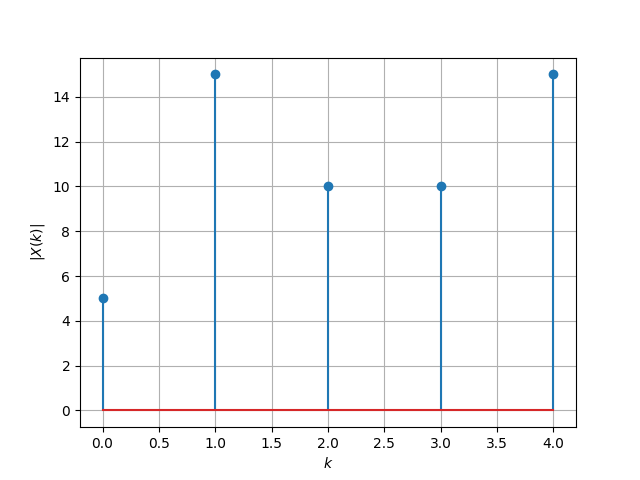
\includegraphics[width=\columnwidth]{2023/EC/47/figs/mm1.png}
    \caption{Amplitude of equation \eqref{eq:gate23ec47eq3}}
    \label{fig:gate23ec47fig1}
\end{figure}
\begin{figure}[htbp]
    \centering
    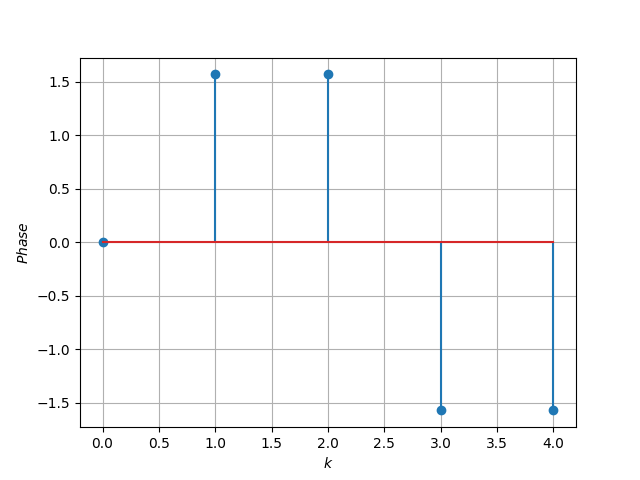
\includegraphics[width=\columnwidth]{2023/EC/47/figs/mm11.png}
    \caption{Phase of equation \eqref{eq:gate23ec47eq3}}
    \label{fig:gate23ec47fig2}
\end{figure}

\item Solving the question for N=8:
\begin{table}[h!]
 	\centering
 	\resizebox{6 cm}{!}{
 		\begin{tabular}{|c|c|c|}
    \hline
    \textbf{Parameter} & \textbf{Value} & \textbf{Description} \\[6pt]
    \hline
    $N$ &  $8$ & Time period \\ \cline{1-2}\cline{3-3}
    $X(k)$ &  $\sum\limits_{n=0}^{N-1} x(n)e^{\frac{-j2\pi kn}{N}}$ & DFT formula\\ \cline{1-2}\cline{3-3}
    $X(0)$ &  $8$ & \multirow{5}{*}{\begin{tabular}[c]{@{}c@{}}DFT \\ values\end{tabular}} \\ \cline{1-2}
    $X(1)$ &  $24j$ &    \\ \cline{1-2}
    $X(2)$ &  $16j$ &    \\ \cline{1-2}
    $X(3)$ &  $-16j$ &    \\ \cline{1-2}
    $X(4)$ &  $-24j$ &    \\ \cline{1-2}
    $X(5)$ &  $0$ &    \\ \cline{1-2}
    $X(6)$ &  $0$ &    \\ \cline{1-2}
    $X(7)$ &  $0$ &    \\ \hline
\end{tabular}

 	}
 	\vspace{6 pt}
 	\caption{Input Parameters}
 	\label{tab:gate23ec47tab1}
 \end{table} 
\begin{align}
\sum\limits_{n=0}^{7}x(n) \sin\brak{\frac{4\pi n}{8}}&=\sum\limits_{n=0}^{7}x(n)\sbrak{\frac{e^{\frac{j4\pi n}{8}}-e^{\frac{-j4\pi n}{8}}}{2j}}\\
&=\frac{1}{2j}\sbrak{\sum\limits_{n=0}^{7}x(n)e^{\frac{j2\pi (2)n}{8}}-\sum\limits_{n=0}^{7}x(n)e^{\frac{-j2\pi (2)n}{8}}}\label{eq:gate23ec47eq9}
\end{align}

Refering to the table \ref{tab:gate23ec47tab1}.
\begin{align}
X(k)&=\sum\limits_{n=0}^{7} x(n)e^{\frac{-j2\pi kn}{8}}\label{eq:gate23ec47eq10}
\end{align}
Referencing from equation\eqref{eq:gate23ec47eq10}, equation\eqref{eq:gate23ec47eq9} can be written as:
\begin{align}
\sum\limits_{n=0}^{7}x(n) \sin\brak{\frac{4\pi n}{8}}&=\frac{1}{2j}\sbrak{X(-2)-X(2)}\label{eq:gate23ec47eq11}
\end{align}
From the property of discrete Fourier series.\\
\begin{align}
X(k)=X(k+N)
\end{align}
So, equation\eqref{eq:gate23ec47eq11} becomes,\\
\begin{align}
\sum\limits_{n=0}^{7}x(n) \sin\brak{\frac{4\pi n}{8}}&=\frac{1}{2j}\sbrak{X(6)-X(2)}\\
\sum\limits_{n=0}^{7}x(n) \sin\brak{\frac{4\pi n}{8}}&=-8
\end{align}
\begin{figure}[h!]
    \centering
    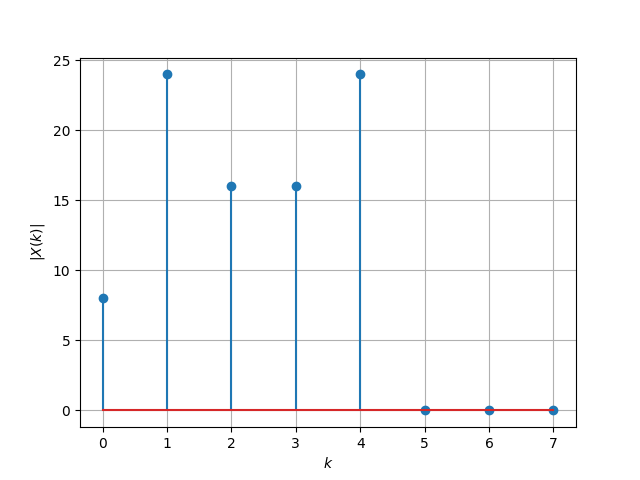
\includegraphics[width=\columnwidth]{2023/EC/47/figs/mm2.png}
    \caption{Amplitude of equation \eqref{eq:gate23ec47eq10}}
    \label{fig:gate23ec47fig3}
\end{figure}
\begin{figure}[h!]
    \centering
    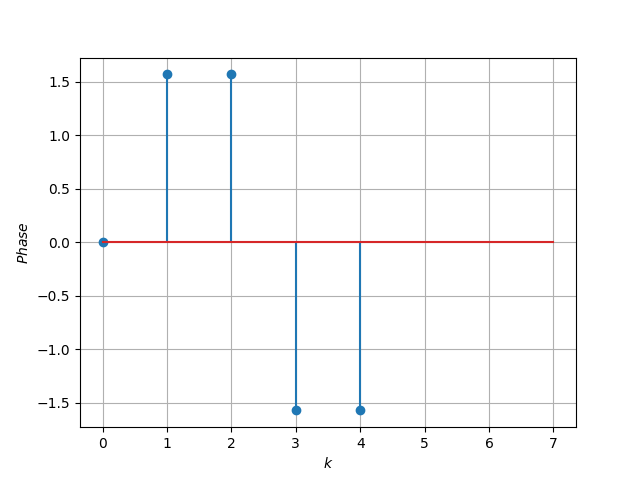
\includegraphics[width=\columnwidth]{2023/EC/47/figs/mm21.png}
    \caption{Phase of equation \eqref{eq:gate23ec47eq10}}
    \label{fig:gate23ec47fig4}
\end{figure}

\end{enumerate}

%\end{document}

\newpage

\item The continuous time signal $x(t)$ is described by:
\begin{align}
x(t)=
    \begin{cases}
        1, & \text{if } 0\: {\displaystyle \leq }\:t\:{\displaystyle \leq }\:1\\
        0, & \text{elsewhere}
    \end{cases} 
\end{align}
If $y(t)$ represents $x(t)$ convolved with itself, which of the following options is/are TRUE?
\begin{enumerate}[label = \Alph*]
    \item $y(t)$ = 0 for all $t<0$\\
    \item $y(t)$ = 0 for all $t>1$\\
    \item $y(t)$ = 0 for all $t>3$\\
    \item $\int_{0.1}^{0.75} \frac{dy(t)}{dt}\: \text{dt} \neq 0$
\end{enumerate}
\solution
\newpage

\item The Z-transform of a discrete signal $x\brak{n}$ is
\begin{align}
X\brak{z}=\dfrac{4z}{\brak{z-\dfrac{1}{5}} \brak{z-\dfrac{2}{3}} \brak{z-3}} \text{ with ROC= }R
\end{align}
Which one of the following statements is TRUE?
\begin{enumerate}[label = (\alph*)]
     \item Discrete time Fourier transform of $x\sbrak{n}$ converges if $R$ is $|z|>3$\\
     \item Discrete time Fourier transform of $x\sbrak{n}$ converges if $ R$ is $\dfrac{2}{3}<|z|<3$\\
     \item Discrete time Fourier transform of $x\sbrak{n}$ converges if $R$ is such that $x\sbrak{n}$ is a left-sided sequence.\\
     \item Discrete time Fourier transform of $x\sbrak{n}$ converges if $R$ is such that $x\sbrak{n}$is a right-sided sequence.\\
 \end{enumerate} \hfill{GATE EE 2023}	\\
 \solution
 \input{2023/EE/19/1.tex}
 \newpage
 
\item The phase margin of the transfer function $G(s) = \frac{2(1-s)}{(1+s)^2}$ is \rule{1cm}{0.15mm} degrees. (rounded off to the nearest integer). \hfill (GATE IN 2023)\\
\solution
\input{2023/IN/50/in_50.tex}
\newpage
\item Consider the second-order linear differential equation
\[x^2\frac{d^2y}{dx^2}+x\frac{dy}{dx}-y=0, \; x\geq 1\]
with the initial conditions \[y(x=1)=6,\; \;\; \frac{dy}{dx}\big{|}_{x=1}=2.\]
Then the value of $y$ at $x=2$ is \rule{2cm}{0.1mm}.\\{\hfill{GATE ME 2023}}\\
\solution
\iffalse
\let\negmedspace\undefined
\let\negthickspace\undefined
\documentclass[journal,12pt,twocolumn]{IEEEtran}
\usepackage{cite}
\usepackage{amsmath,amssymb,amsfonts,amsthm}
\usepackage{algorithmic}
\usepackage{graphicx}
\usepackage{textcomp}
\usepackage{xcolor}
\usepackage{txfonts}
\usepackage{listings}
\usepackage{enumitem}
\usepackage{mathtools}
\usepackage{gensymb}
\usepackage{comment}
\usepackage[breaklinks=true]{adjustbox}
\usepackage{tkz-euclide} 
\usepackage{listings}
\usepackage{gvv}                                        
\def\inputGnumericTable{}                                 
\usepackage[latin1]{inputenc}                                
\usepackage{color}                                            
\usepackage{array}                                            
\usepackage{longtable}                                       
\usepackage{calc}                                             
\usepackage{multirow}                                         
\usepackage{hhline}                                           
\usepackage{ifthen}                                           
\usepackage{lscape}

\newtheorem{theorem}{Theorem}[section]
\newtheorem{problem}{Problem}
\newtheorem{proposition}{Proposition}[section]
\newtheorem{lemma}{Lemma}[section]
\newtheorem{corollary}[theorem]{Corollary}
\newtheorem{example}{Example}[section]
\newtheorem{definition}[problem]{Definition}
\newcommand{\BEQA}{\begin{eqnarray}}
\newcommand{\EEQA}{\end{eqnarray}}
\newcommand{\define}{\stackrel{\triangle}{=}}
\theoremstyle{remark}
\newtheorem{rem}{Remark}

\begin{document}
\bibliographystyle{IEEEtran}

\vspace{3cm}

\title{}
\author{EE23BTECH11024 - G.Karthik Yadav$^{*}$
}
\maketitle
\newpage
\bigskip

\section*{GATE 2023 EC 41}
\noindent 1. \hspace{2pt} A Closed loop systen is shown in the figure where $k>0$ and $\alpha>0$ .\\
The Steady State error due to a ramp input $\brak{R\brak{s} = \alpha s^{-2}}$ is given by \hfill{(GATE 2023 EC 41)}

\begin{figure}[ht]
\centering
    \includegraphics[width=1.0\linewidth]{2023/EC/41/figs/question.png}
    \label{fig: 23.EC.41.24.1}
\end{figure}

\begin{enumerate}
\item $\frac{2\alpha}{k}$
\item $\frac{\alpha}{k}$
\item $\frac{\alpha}{2k}$
\item $\frac{\alpha}{4k}$
\end{enumerate}

\solution\\
\fi
\begin{table}[ht]
\setlength{\arrayrulewidth}{0.3mm}
\setlength{\tabcolsep}{15pt}
\renewcommand{\arraystretch}{1.5}



\begin{tabular}{ |p{1cm}|p{3cm}|p{1cm}| }
\hline
Symbol & Parameters & Value\\
\hline
$R\brak{s}$ & Laplace transform Ramp input signal r\brak{t} &  $\alpha s^{-2}$\\
\hline
$G\brak{s}$ & Open Loop transfer function &  $ \frac{Y\brak{s}}{E\brak{s}} = \frac{k}{s\brak{s+2}}$\\
\hline
$Y\brak{s}$ & Laplace transform of the output signal y\brak{t}  &  ? \\
\hline
$E\brak{s}$ & Laplace transform of the error signal e\brak{t} & R\brak{s} - Y\brak{s}\\
\hline
$E\brak{s}$ & Laplace transform of the error signal e\brak{t} & R\brak{s} - Y\brak{s}\\   
\hline
$e_s$ & Steady State Error &  ? \\
\hline
%$x(l)$ & Last($l^{th}$) term of series & 350\\
%$x(0)$ & Starting ($0^{th}$) term of series & 17 %\\
%\hline
%d & Common difference of AP & 9\\
%\hline
\end{tabular}
\caption{Parameters}






\end{table}
\bigskip
from table  Open loop transfer function $G\brak{s}$\\
\begin{align}
	G\brak{s} &= \frac{Y\brak{s}}{E\brak{s}} \label{24.2023.EC.41.1} \\
        &= \frac{Y\brak{s}}{R\brak{s} - Y\brak{s}} \\
        Y\brak{s} &= \frac{R\brak{s}G\brak{s}}{1 + G\brak{s}} \label{24.2023.EC.41.2}
\end{align}

from eq \ref{24.2023.EC.41.1} and eq \eqref{24.2023.EC.41.2}

\begin{align}
        G\brak{s} &= \frac{k}{s\brak{s +2}}  \label{24.2023.EC.41.3} \\ 
        Y\brak{s} &= \frac{\alpha k s^{-2}}{k + s\brak{s+2}} \label{24.2023.EC.41.4} \\
        E\brak{s} &= R\brak{s} - Y\brak{s}  \label{24.2023.EC.41.5} \\ 
        E\brak{s} &= \frac{\alpha \brak{s+2}}{s\brak{k + s\brak{s+2}}}
\end{align}

By Taking Inverse Laplace Transform of eq \eqref{24.2023.EC.41.3} and eq\eqref{24.2023.EC.41.4}

\begin{align}
    g\brak{t} &= \frac{k\brak{1 - e^{-2t}}}{2} u\brak{t} \\
        y\brak{t} &= \alpha t u\brak{t}- \frac{2\alpha}{k}u\brak{t} \\
        \notag &+\frac{\alpha}{2k\sqrt{1-k}} \biggl(2\sqrt{1-k}e^{\sqrt{1-k}t-1}\\ 
        \notag &+ 2\sqrt{1-k}e^{-\sqrt{1-k}t-1} \\
        \notag &+ \brak{2-k}e^{\sqrt{1-k}t-1} - \brak{2-k}e^{-\sqrt{1-k}t-1} \biggr) u\brak{t}
\end{align}

\begin{align}
        e\brak{t} &= r\brak{t} - y\brak{t} \\
        &= \alpha t u\brak{t} - y\brak{t} \\
        e\brak{t} &= \frac{2\alpha}{k}u\brak{t} \\
        \notag &-\frac{\alpha}{2k\sqrt{1-k}} \biggl(2\sqrt{1-k}e^{\sqrt{1-k}t-1}\\ 
        \notag &+ 2\sqrt{1-k}e^{-\sqrt{1-k}t-1} \\
        \notag &+ \brak{2-k}e^{\sqrt{1-k}t-1} - \brak{2-k}e^{-\sqrt{1-k}t-1} \biggr) u\brak{t}
\end{align}
	

\begin{align}
    e_s &= \displaystyle\lim_{s\to 0}s E\brak{s} \\
    &= \displaystyle\lim_{s\to 0} s \frac{R\brak{s}}{1 + G\brak{s}} \\
    &= \displaystyle\lim_{s\to 0} \frac{\alpha \brak{s+2}}{s\brak{s+2} + k} \\
    e_s &= \frac{2\alpha}{k}
\end{align}



\newpage
\item The transfer function of a measuring instrument is \\
$$G_m(s) = \frac{1.05}{2s+1}exp(-s)$$
At time $t = 0$, a step change of +1 unit is introduced in the input of this instrument.The time taken by the instrument to show an increase of 1 unit in its output is(rounded off to two decimal places).\\ \hfill (GATE CH 2023)
\solution
\iffalse
\let\negmedspace\undefined
\let\negthickspace\undefined
\documentclass[journal,12pt,twocolumn]{IEEEtran}
\usepackage{cite}
\usepackage{amsmath,amssymb,amsfonts,amsthm}
\usepackage{algorithmic}
\usepackage{graphicx}
\usepackage{textcomp}
\usepackage{xcolor}
\usepackage{txfonts}
\usepackage{listings}
\usepackage{enumitem}
\usepackage{mathtools}
\usepackage{gensymb}
\usepackage{comment}
\usepackage[breaklinks=true]{adjustbox}
\usepackage{tkz-euclide} 
\usepackage{listings}
\usepackage{gvv}                                        
\def\inputGnumericTable{}                                 
\usepackage[latin1]{inputenc}                                
\usepackage{color}                                            
\usepackage{array}                                            
\usepackage{longtable}                                       
\usepackage{calc}                                             
\usepackage{multirow}                                         
\usepackage{hhline}                                           
\usepackage{ifthen}                                           
\usepackage{lscape}

\newtheorem{theorem}{Theorem}[section]
\newtheorem{problem}{Problem}
\newtheorem{proposition}{Proposition}[section]
\newtheorem{lemma}{Lemma}[section]
\newtheorem{corollary}[theorem]{Corollary}
\newtheorem{example}{Example}[section]
\newtheorem{definition}[problem]{Definition}
\newcommand{\BEQA}{\begin{eqnarray}}
\newcommand{\EEQA}{\end{eqnarray}}
\newcommand{\define}{\stackrel{\triangle}{=}}
\theoremstyle{remark}
\newtheorem{rem}{Remark}

\begin{document}
\bibliographystyle{IEEEtran}

\vspace{3cm}

\title{}
\author{EE23BTECH11024 - G.Karthik Yadav$^{*}$
}
\maketitle
\newpage
\bigskip

\section*{GATE 2023 EC 41}
\noindent 1. \hspace{2pt} A Closed loop systen is shown in the figure where $k>0$ and $\alpha>0$ .\\
The Steady State error due to a ramp input $\brak{R\brak{s} = \alpha s^{-2}}$ is given by \hfill{(GATE 2023 EC 41)}

\begin{figure}[ht]
\centering
    \includegraphics[width=1.0\linewidth]{2023/EC/41/figs/question.png}
    \label{fig: 23.EC.41.24.1}
\end{figure}

\begin{enumerate}
\item $\frac{2\alpha}{k}$
\item $\frac{\alpha}{k}$
\item $\frac{\alpha}{2k}$
\item $\frac{\alpha}{4k}$
\end{enumerate}

\solution\\
\fi
\begin{table}[ht]
\setlength{\arrayrulewidth}{0.3mm}
\setlength{\tabcolsep}{15pt}
\renewcommand{\arraystretch}{1.5}



\begin{tabular}{ |p{1cm}|p{3cm}|p{1cm}| }
\hline
Symbol & Parameters & Value\\
\hline
$R\brak{s}$ & Laplace transform Ramp input signal r\brak{t} &  $\alpha s^{-2}$\\
\hline
$G\brak{s}$ & Open Loop transfer function &  $ \frac{Y\brak{s}}{E\brak{s}} = \frac{k}{s\brak{s+2}}$\\
\hline
$Y\brak{s}$ & Laplace transform of the output signal y\brak{t}  &  ? \\
\hline
$E\brak{s}$ & Laplace transform of the error signal e\brak{t} & R\brak{s} - Y\brak{s}\\
\hline
$E\brak{s}$ & Laplace transform of the error signal e\brak{t} & R\brak{s} - Y\brak{s}\\   
\hline
$e_s$ & Steady State Error &  ? \\
\hline
%$x(l)$ & Last($l^{th}$) term of series & 350\\
%$x(0)$ & Starting ($0^{th}$) term of series & 17 %\\
%\hline
%d & Common difference of AP & 9\\
%\hline
\end{tabular}
\caption{Parameters}






\end{table}
\bigskip
from table  Open loop transfer function $G\brak{s}$\\
\begin{align}
	G\brak{s} &= \frac{Y\brak{s}}{E\brak{s}} \label{24.2023.EC.41.1} \\
        &= \frac{Y\brak{s}}{R\brak{s} - Y\brak{s}} \\
        Y\brak{s} &= \frac{R\brak{s}G\brak{s}}{1 + G\brak{s}} \label{24.2023.EC.41.2}
\end{align}

from eq \ref{24.2023.EC.41.1} and eq \eqref{24.2023.EC.41.2}

\begin{align}
        G\brak{s} &= \frac{k}{s\brak{s +2}}  \label{24.2023.EC.41.3} \\ 
        Y\brak{s} &= \frac{\alpha k s^{-2}}{k + s\brak{s+2}} \label{24.2023.EC.41.4} \\
        E\brak{s} &= R\brak{s} - Y\brak{s}  \label{24.2023.EC.41.5} \\ 
        E\brak{s} &= \frac{\alpha \brak{s+2}}{s\brak{k + s\brak{s+2}}}
\end{align}

By Taking Inverse Laplace Transform of eq \eqref{24.2023.EC.41.3} and eq\eqref{24.2023.EC.41.4}

\begin{align}
    g\brak{t} &= \frac{k\brak{1 - e^{-2t}}}{2} u\brak{t} \\
        y\brak{t} &= \alpha t u\brak{t}- \frac{2\alpha}{k}u\brak{t} \\
        \notag &+\frac{\alpha}{2k\sqrt{1-k}} \biggl(2\sqrt{1-k}e^{\sqrt{1-k}t-1}\\ 
        \notag &+ 2\sqrt{1-k}e^{-\sqrt{1-k}t-1} \\
        \notag &+ \brak{2-k}e^{\sqrt{1-k}t-1} - \brak{2-k}e^{-\sqrt{1-k}t-1} \biggr) u\brak{t}
\end{align}

\begin{align}
        e\brak{t} &= r\brak{t} - y\brak{t} \\
        &= \alpha t u\brak{t} - y\brak{t} \\
        e\brak{t} &= \frac{2\alpha}{k}u\brak{t} \\
        \notag &-\frac{\alpha}{2k\sqrt{1-k}} \biggl(2\sqrt{1-k}e^{\sqrt{1-k}t-1}\\ 
        \notag &+ 2\sqrt{1-k}e^{-\sqrt{1-k}t-1} \\
        \notag &+ \brak{2-k}e^{\sqrt{1-k}t-1} - \brak{2-k}e^{-\sqrt{1-k}t-1} \biggr) u\brak{t}
\end{align}
	

\begin{align}
    e_s &= \displaystyle\lim_{s\to 0}s E\brak{s} \\
    &= \displaystyle\lim_{s\to 0} s \frac{R\brak{s}}{1 + G\brak{s}} \\
    &= \displaystyle\lim_{s\to 0} \frac{\alpha \brak{s+2}}{s\brak{s+2} + k} \\
    e_s &= \frac{2\alpha}{k}
\end{align}



\newpage
\item
The laplace transform of $x_1(t)$ = $e^{-t}u(t)$ is $X_1(s)$, where $u(t)$ is the unit step function. The laplace transform of $x_2(t) = e^tu(-t)$ is $X_2(s)$. Which one of the following statements is TRUE?
\begin{enumerate}
    \item The region of convergence of $X_1(s)$ is $Re(s) \geq 0$
    \item The region of convergence of $X_2(s)$ is confined to the left half-plane of s.
    \item The region of convergence of $X_1(s)$ is confined to the right half-plane of s.
    \item the imaginary axis in the s-plane is included in both the region of convergence of $X_1(s)$ and the region of convergence of $X_2(s)$.
\end{enumerate} \hfill(GATE BM 2023)\\
\solution
\input{2023/BM/39/bm39.tex}
\newpage
\item Given that $\frac{dy}{dx}=2x+y$ and $y=1$,when $x=0$ Using Runge-Kutta fourth order method,the value of $y$ at $x=0.2$ is \hfill(GATE 2023 AG 50) \\
\solution
\iffalse
\let\negmedspace\undefined
\let\negthickspace\undefined
\documentclass[journal,12pt,twocolumn]{IEEEtran}
\usepackage{cite}
\usepackage{amsmath,amssymb,amsfonts,amsthm}
\usepackage{algorithmic}
\usepackage{graphicx}
\usepackage{textcomp}
\usepackage{xcolor}
\usepackage{txfonts}
\usepackage{listings}
\usepackage{enumitem}
\usepackage{mathtools}
\usepackage{gensymb}
\usepackage{comment}
\usepackage[breaklinks=true]{hyperref}
\usepackage{tkz-euclide} 
\usepackage{listings}
\usepackage{gvv}                                        
\def\inputGnumericTable{}                                 
\usepackage[latin1]{inputenc}                                
\usepackage{color}                                            
\usepackage{array}                                            
\usepackage{longtable}                                       
\usepackage{calc}                                             
\usepackage{multirow}                                         
\usepackage{hhline}                                           
\usepackage{ifthen}                                           
\usepackage{lscape}
\usepackage{caption}
\newtheorem{theorem}{Theorem}[section]
\newtheorem{problem}{Problem}
\newtheorem{proposition}{Proposition}[section]
\newtheorem{lemma}{Lemma}[section]
\newtheorem{corollary}[theorem]{Corollary}
\newtheorem{example}{Example}[section]
\newtheorem{definition}[problem]{Definition}
\newcommand{\BEQA}{\begin{eqnarray}}
\newcommand{\EEQA}{\end{eqnarray}}
\newcommand{\define}{\stackrel{\triangle}{=}}
\theoremstyle{remark}
\newtheorem{rem}{Remark}
\begin{document}

\bibliographystyle{IEEEtran}
\vspace{3cm}

\title{10.5.2.14}
\author{EE23BTECH11003 - pranav}
\maketitle
\newpage

\bigskip
\renewcommand{\thefigure}{\arabic{figure}}
\renewcommand{\thetable}{\arabic{table}}

\textbf{Question}:Given that $\frac{dy}{dx}=2x+y$ and $y=1$,when $x=0$ Using Runge-Kutta fourth order method,the value of $y$ at $x=0.2$ is \hfill(GATE 2023 AG 50) 
\solution
\fi
By using runge kutta 4 th order method\\
\begin{table}[h]
    \centering
    \input{2023/AG/50/tables/Table.Tex}
    \caption{Variables Used}
\end{table}
\begin{align}
y(n)=y(n-1)+\frac{h}{6}[(2x(n-1)+y(n-1)(6+3h+h^2+\frac{h^3}{4})+(6h+2h^2+\frac{h^3}{2})]
\end{align}
assume step size as $0.1$ and initial conditions as $x=0$ and $y=1$\\
\begin{align}
y(n)&=1+(6+3(0.1)+0.1^2+\frac{0.1^3}{4})+(6(0.1)+2(0.1)^2+\frac{0.1^3}{2})\\
\implies y_{n}&=1.115
\end{align}
cosidering outputs of last iteration as inputs of next iteration\\
\begin{align}
y(n)=1.155+\frac{0.1}{6}[(2(0.1)+1.155(6+3(0.1)+(0.1)^2+\frac{(0.1)^3}{4})+(6(0.1)+2(0.1)^2+\frac{(0.1)^3}{2})]
\implies y(n)=1.29
\end{align}
so at $x=0.2$ value of $y$ is $1.29$\\
analysis
\begin{align}
\frac{dy}{dx}&=2x+y\\
ye^{-x}&=\int2xe^{-x}dx\\
\implies ye^{-x}&=-2(x+1)e^{-x}+c
\end{align}
by using intial conditions
\begin{align}
c=3\\
\implies y=3e^x-2(x+1)
\end{align}
\newpage
\begin{figure}
    \centering
    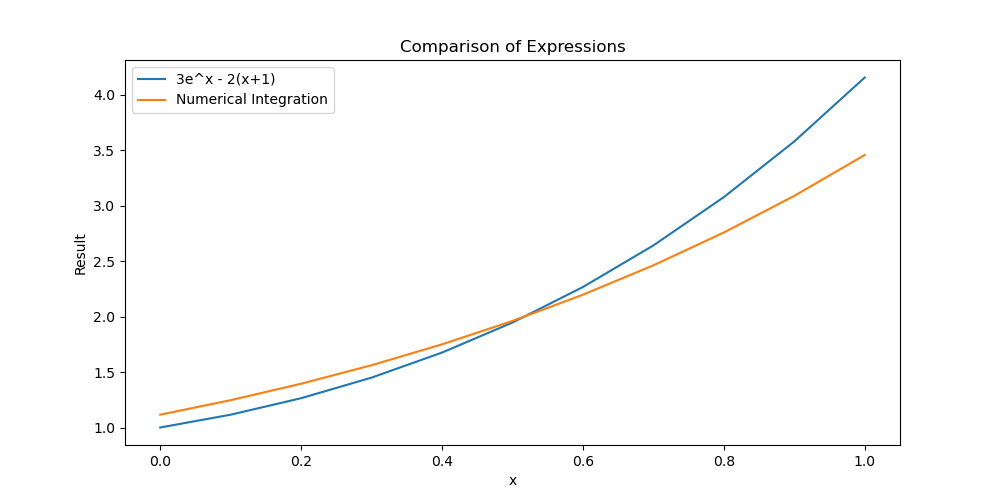
\includegraphics[width=1\linewidth]{2023/AG/50/figs/grap.png}
    \caption{simulation vs analysis}
\end{figure}

%\end{document}

\item The magnitude and phase plots shown in the figure match with the transfer-
function
\begin{figure}[h]
    \centering
    \includegraphics[width=\columnwidth]{2023/IN/43/figs/question.png}
\end{figure}\\
\begin{enumerate}
\item $\frac{10000}{s^2+2s+10000}$\\
\item $\frac{10000}{s^2+2s+10000}e^{-0.05s}$\\
\item $\frac{10000}{s^2+2s+10000}e^{-0.5\times10^{-12}s}$\\
\item $\frac{100}{s^2+2s+100}$
\end{enumerate}
\hfill{(GATE IN 2023)}
\solution
\iffalse
\let\negmedspace\undefined
\let\negthickspace\undefined
\documentclass[journal,12pt,twocolumn]{IEEEtran}
\usepackage{cite}
\usepackage{amsmath,amssymb,amsfonts,amsthm}
\usepackage{algorithmic}
\usepackage{graphicx}
\usepackage{textcomp}
\usepackage{xcolor}
\usepackage{txfonts}
\usepackage{listings}
\usepackage{enumitem}
\usepackage{mathtools}
\usepackage{gensymb}
\usepackage{comment}
\usepackage[breaklinks=true]{adjustbox}
\usepackage{tkz-euclide} 
\usepackage{listings}
\usepackage{gvv}                                        
\def\inputGnumericTable{}                                 
\usepackage[latin1]{inputenc}                                
\usepackage{color}                                            
\usepackage{array}                                            
\usepackage{longtable}                                       
\usepackage{calc}                                             
\usepackage{multirow}                                         
\usepackage{hhline}                                           
\usepackage{ifthen}                                           
\usepackage{lscape}

\newtheorem{theorem}{Theorem}[section]
\newtheorem{problem}{Problem}
\newtheorem{proposition}{Proposition}[section]
\newtheorem{lemma}{Lemma}[section]
\newtheorem{corollary}[theorem]{Corollary}
\newtheorem{example}{Example}[section]
\newtheorem{definition}[problem]{Definition}
\newcommand{\BEQA}{\begin{eqnarray}}
\newcommand{\EEQA}{\end{eqnarray}}
\newcommand{\define}{\stackrel{\triangle}{=}}
\theoremstyle{remark}
\newtheorem{rem}{Remark}

\begin{document}
\bibliographystyle{IEEEtran}

\vspace{3cm}

\title{}
\author{EE23BTECH11024 - G.Karthik Yadav$^{*}$
}
\maketitle
\newpage
\bigskip

\section*{GATE 2023 EC 41}
\noindent 1. \hspace{2pt} A Closed loop systen is shown in the figure where $k>0$ and $\alpha>0$ .\\
The Steady State error due to a ramp input $\brak{R\brak{s} = \alpha s^{-2}}$ is given by \hfill{(GATE 2023 EC 41)}

\begin{figure}[ht]
\centering
    \includegraphics[width=1.0\linewidth]{2023/EC/41/figs/question.png}
    \label{fig: 23.EC.41.24.1}
\end{figure}

\begin{enumerate}
\item $\frac{2\alpha}{k}$
\item $\frac{\alpha}{k}$
\item $\frac{\alpha}{2k}$
\item $\frac{\alpha}{4k}$
\end{enumerate}

\solution\\
\fi
\begin{table}[ht]
\setlength{\arrayrulewidth}{0.3mm}
\setlength{\tabcolsep}{15pt}
\renewcommand{\arraystretch}{1.5}



\begin{tabular}{ |p{1cm}|p{3cm}|p{1cm}| }
\hline
Symbol & Parameters & Value\\
\hline
$R\brak{s}$ & Laplace transform Ramp input signal r\brak{t} &  $\alpha s^{-2}$\\
\hline
$G\brak{s}$ & Open Loop transfer function &  $ \frac{Y\brak{s}}{E\brak{s}} = \frac{k}{s\brak{s+2}}$\\
\hline
$Y\brak{s}$ & Laplace transform of the output signal y\brak{t}  &  ? \\
\hline
$E\brak{s}$ & Laplace transform of the error signal e\brak{t} & R\brak{s} - Y\brak{s}\\
\hline
$E\brak{s}$ & Laplace transform of the error signal e\brak{t} & R\brak{s} - Y\brak{s}\\   
\hline
$e_s$ & Steady State Error &  ? \\
\hline
%$x(l)$ & Last($l^{th}$) term of series & 350\\
%$x(0)$ & Starting ($0^{th}$) term of series & 17 %\\
%\hline
%d & Common difference of AP & 9\\
%\hline
\end{tabular}
\caption{Parameters}






\end{table}
\bigskip
from table  Open loop transfer function $G\brak{s}$\\
\begin{align}
	G\brak{s} &= \frac{Y\brak{s}}{E\brak{s}} \label{24.2023.EC.41.1} \\
        &= \frac{Y\brak{s}}{R\brak{s} - Y\brak{s}} \\
        Y\brak{s} &= \frac{R\brak{s}G\brak{s}}{1 + G\brak{s}} \label{24.2023.EC.41.2}
\end{align}

from eq \ref{24.2023.EC.41.1} and eq \eqref{24.2023.EC.41.2}

\begin{align}
        G\brak{s} &= \frac{k}{s\brak{s +2}}  \label{24.2023.EC.41.3} \\ 
        Y\brak{s} &= \frac{\alpha k s^{-2}}{k + s\brak{s+2}} \label{24.2023.EC.41.4} \\
        E\brak{s} &= R\brak{s} - Y\brak{s}  \label{24.2023.EC.41.5} \\ 
        E\brak{s} &= \frac{\alpha \brak{s+2}}{s\brak{k + s\brak{s+2}}}
\end{align}

By Taking Inverse Laplace Transform of eq \eqref{24.2023.EC.41.3} and eq\eqref{24.2023.EC.41.4}

\begin{align}
    g\brak{t} &= \frac{k\brak{1 - e^{-2t}}}{2} u\brak{t} \\
        y\brak{t} &= \alpha t u\brak{t}- \frac{2\alpha}{k}u\brak{t} \\
        \notag &+\frac{\alpha}{2k\sqrt{1-k}} \biggl(2\sqrt{1-k}e^{\sqrt{1-k}t-1}\\ 
        \notag &+ 2\sqrt{1-k}e^{-\sqrt{1-k}t-1} \\
        \notag &+ \brak{2-k}e^{\sqrt{1-k}t-1} - \brak{2-k}e^{-\sqrt{1-k}t-1} \biggr) u\brak{t}
\end{align}

\begin{align}
        e\brak{t} &= r\brak{t} - y\brak{t} \\
        &= \alpha t u\brak{t} - y\brak{t} \\
        e\brak{t} &= \frac{2\alpha}{k}u\brak{t} \\
        \notag &-\frac{\alpha}{2k\sqrt{1-k}} \biggl(2\sqrt{1-k}e^{\sqrt{1-k}t-1}\\ 
        \notag &+ 2\sqrt{1-k}e^{-\sqrt{1-k}t-1} \\
        \notag &+ \brak{2-k}e^{\sqrt{1-k}t-1} - \brak{2-k}e^{-\sqrt{1-k}t-1} \biggr) u\brak{t}
\end{align}
	

\begin{align}
    e_s &= \displaystyle\lim_{s\to 0}s E\brak{s} \\
    &= \displaystyle\lim_{s\to 0} s \frac{R\brak{s}}{1 + G\brak{s}} \\
    &= \displaystyle\lim_{s\to 0} \frac{\alpha \brak{s+2}}{s\brak{s+2} + k} \\
    e_s &= \frac{2\alpha}{k}
\end{align}



\newpage
\item The Laplace transform of the continuous-time signal $x\brak{t} = e^{-3t}u\brak{t - 5}$ is 
\rule{1cm}{0.15mm}, where $u\brak{t}$ denotes the continuous-time unit step signal.

\begin{enumerate}[label = \Alph*)]
    \item $\frac{e^{-5s}}{s + 3}$, Real$\{s\} > -3$\\
    \item $\frac{e^{-5(s - 3)}}{s - 3}$, Real$\{s\} > 3$\\
    \item $\frac{e^{-5(s + 3)}}{s + 3}$, Real$\{s\} > -3$\\
    \item $\frac{e^{-5(s - 3)}}{s + 3}$, Real$\{s\} > -3$\\
\end{enumerate}
\solution
\iffalse
\let\negmedspace\undefined
\let\negthickspace\undefined
\documentclass[journal,12pt,twocolumn]{IEEEtran}
\usepackage{cite}
\usepackage{amsmath,amssymb,amsfonts,amsthm}
\usepackage{algorithmic}
\usepackage{graphicx}
\usepackage{textcomp}
\usepackage{xcolor}
\usepackage{txfonts}
\usepackage{listings}
\usepackage{enumitem}
\usepackage{mathtools}
\usepackage{gensymb}
\usepackage{comment}
\usepackage[breaklinks=true]{adjustbox}
\usepackage{tkz-euclide} 
\usepackage{listings}
\usepackage{gvv}                                        
\def\inputGnumericTable{}                                 
\usepackage[latin1]{inputenc}                                
\usepackage{color}                                            
\usepackage{array}                                            
\usepackage{longtable}                                       
\usepackage{calc}                                             
\usepackage{multirow}                                         
\usepackage{hhline}                                           
\usepackage{ifthen}                                           
\usepackage{lscape}

\newtheorem{theorem}{Theorem}[section]
\newtheorem{problem}{Problem}
\newtheorem{proposition}{Proposition}[section]
\newtheorem{lemma}{Lemma}[section]
\newtheorem{corollary}[theorem]{Corollary}
\newtheorem{example}{Example}[section]
\newtheorem{definition}[problem]{Definition}
\newcommand{\BEQA}{\begin{eqnarray}}
\newcommand{\EEQA}{\end{eqnarray}}
\newcommand{\define}{\stackrel{\triangle}{=}}
\theoremstyle{remark}
\newtheorem{rem}{Remark}

\begin{document}
\bibliographystyle{IEEEtran}

\vspace{3cm}

\title{}
\author{EE23BTECH11024 - G.Karthik Yadav$^{*}$
}
\maketitle
\newpage
\bigskip

\section*{GATE 2023 EC 41}
\noindent 1. \hspace{2pt} A Closed loop systen is shown in the figure where $k>0$ and $\alpha>0$ .\\
The Steady State error due to a ramp input $\brak{R\brak{s} = \alpha s^{-2}}$ is given by \hfill{(GATE 2023 EC 41)}

\begin{figure}[ht]
\centering
    \includegraphics[width=1.0\linewidth]{2023/EC/41/figs/question.png}
    \label{fig: 23.EC.41.24.1}
\end{figure}

\begin{enumerate}
\item $\frac{2\alpha}{k}$
\item $\frac{\alpha}{k}$
\item $\frac{\alpha}{2k}$
\item $\frac{\alpha}{4k}$
\end{enumerate}

\solution\\
\fi
\begin{table}[ht]
\setlength{\arrayrulewidth}{0.3mm}
\setlength{\tabcolsep}{15pt}
\renewcommand{\arraystretch}{1.5}



\begin{tabular}{ |p{1cm}|p{3cm}|p{1cm}| }
\hline
Symbol & Parameters & Value\\
\hline
$R\brak{s}$ & Laplace transform Ramp input signal r\brak{t} &  $\alpha s^{-2}$\\
\hline
$G\brak{s}$ & Open Loop transfer function &  $ \frac{Y\brak{s}}{E\brak{s}} = \frac{k}{s\brak{s+2}}$\\
\hline
$Y\brak{s}$ & Laplace transform of the output signal y\brak{t}  &  ? \\
\hline
$E\brak{s}$ & Laplace transform of the error signal e\brak{t} & R\brak{s} - Y\brak{s}\\
\hline
$E\brak{s}$ & Laplace transform of the error signal e\brak{t} & R\brak{s} - Y\brak{s}\\   
\hline
$e_s$ & Steady State Error &  ? \\
\hline
%$x(l)$ & Last($l^{th}$) term of series & 350\\
%$x(0)$ & Starting ($0^{th}$) term of series & 17 %\\
%\hline
%d & Common difference of AP & 9\\
%\hline
\end{tabular}
\caption{Parameters}






\end{table}
\bigskip
from table  Open loop transfer function $G\brak{s}$\\
\begin{align}
	G\brak{s} &= \frac{Y\brak{s}}{E\brak{s}} \label{24.2023.EC.41.1} \\
        &= \frac{Y\brak{s}}{R\brak{s} - Y\brak{s}} \\
        Y\brak{s} &= \frac{R\brak{s}G\brak{s}}{1 + G\brak{s}} \label{24.2023.EC.41.2}
\end{align}

from eq \ref{24.2023.EC.41.1} and eq \eqref{24.2023.EC.41.2}

\begin{align}
        G\brak{s} &= \frac{k}{s\brak{s +2}}  \label{24.2023.EC.41.3} \\ 
        Y\brak{s} &= \frac{\alpha k s^{-2}}{k + s\brak{s+2}} \label{24.2023.EC.41.4} \\
        E\brak{s} &= R\brak{s} - Y\brak{s}  \label{24.2023.EC.41.5} \\ 
        E\brak{s} &= \frac{\alpha \brak{s+2}}{s\brak{k + s\brak{s+2}}}
\end{align}

By Taking Inverse Laplace Transform of eq \eqref{24.2023.EC.41.3} and eq\eqref{24.2023.EC.41.4}

\begin{align}
    g\brak{t} &= \frac{k\brak{1 - e^{-2t}}}{2} u\brak{t} \\
        y\brak{t} &= \alpha t u\brak{t}- \frac{2\alpha}{k}u\brak{t} \\
        \notag &+\frac{\alpha}{2k\sqrt{1-k}} \biggl(2\sqrt{1-k}e^{\sqrt{1-k}t-1}\\ 
        \notag &+ 2\sqrt{1-k}e^{-\sqrt{1-k}t-1} \\
        \notag &+ \brak{2-k}e^{\sqrt{1-k}t-1} - \brak{2-k}e^{-\sqrt{1-k}t-1} \biggr) u\brak{t}
\end{align}

\begin{align}
        e\brak{t} &= r\brak{t} - y\brak{t} \\
        &= \alpha t u\brak{t} - y\brak{t} \\
        e\brak{t} &= \frac{2\alpha}{k}u\brak{t} \\
        \notag &-\frac{\alpha}{2k\sqrt{1-k}} \biggl(2\sqrt{1-k}e^{\sqrt{1-k}t-1}\\ 
        \notag &+ 2\sqrt{1-k}e^{-\sqrt{1-k}t-1} \\
        \notag &+ \brak{2-k}e^{\sqrt{1-k}t-1} - \brak{2-k}e^{-\sqrt{1-k}t-1} \biggr) u\brak{t}
\end{align}
	

\begin{align}
    e_s &= \displaystyle\lim_{s\to 0}s E\brak{s} \\
    &= \displaystyle\lim_{s\to 0} s \frac{R\brak{s}}{1 + G\brak{s}} \\
    &= \displaystyle\lim_{s\to 0} \frac{\alpha \brak{s+2}}{s\brak{s+2} + k} \\
    e_s &= \frac{2\alpha}{k}
\end{align}




\newpage

\item The solution $x\brak{t}$, $t \geq 0$, to the differential equation
$\ddot{x} = -k\dot{x} , k > 0$ with initial conditions $x\brak{0} = 1$ and $\dot{x}\brak{0} = 0$ is
\begin{enumerate}[label = (\Alph*)]
    \item $x\brak{t} = 2e^{-kt} + 2kt -1 $\label{gate.in.20.a} \\
    \item $x\brak{t} = 2e^{-kt} -1 $\label{gate.in.20.b}\\
    \item $x\brak{t} = 1 $\label{gate.in.20.c}\\
    \item $x\brak{t} = 2e^{-kt} - kt - 1 $\label{gate.in.20.d}
\end{enumerate}
\hfill{GATE ~2023  , IN}\\
\solution
\iffalse
\let\negmedspace\undefined
\let\negthickspace\undefined
\documentclass[journal,12pt,twocolumn]{IEEEtran}
\usepackage{cite}
\usepackage{amsmath,amssymb,amsfonts,amsthm}
\usepackage{algorithmic}
\usepackage{graphicx}
\usepackage{textcomp}
\usepackage{xcolor}
\usepackage{txfonts}
\usepackage{listings}
\usepackage{enumitem}
\usepackage{mathtools}
\usepackage{gensymb}
\usepackage{comment}
\usepackage[breaklinks=true]{adjustbox}
\usepackage{tkz-euclide} 
\usepackage{listings}
\usepackage{gvv}                                        
\def\inputGnumericTable{}                                 
\usepackage[latin1]{inputenc}                                
\usepackage{color}                                            
\usepackage{array}                                            
\usepackage{longtable}                                       
\usepackage{calc}                                             
\usepackage{multirow}                                         
\usepackage{hhline}                                           
\usepackage{ifthen}                                           
\usepackage{lscape}

\newtheorem{theorem}{Theorem}[section]
\newtheorem{problem}{Problem}
\newtheorem{proposition}{Proposition}[section]
\newtheorem{lemma}{Lemma}[section]
\newtheorem{corollary}[theorem]{Corollary}
\newtheorem{example}{Example}[section]
\newtheorem{definition}[problem]{Definition}
\newcommand{\BEQA}{\begin{eqnarray}}
\newcommand{\EEQA}{\end{eqnarray}}
\newcommand{\define}{\stackrel{\triangle}{=}}
\theoremstyle{remark}
\newtheorem{rem}{Remark}

\begin{document}
\bibliographystyle{IEEEtran}

\vspace{3cm}

\title{}
\author{EE23BTECH11024 - G.Karthik Yadav$^{*}$
}
\maketitle
\newpage
\bigskip

\section*{GATE 2023 EC 41}
\noindent 1. \hspace{2pt} A Closed loop systen is shown in the figure where $k>0$ and $\alpha>0$ .\\
The Steady State error due to a ramp input $\brak{R\brak{s} = \alpha s^{-2}}$ is given by \hfill{(GATE 2023 EC 41)}

\begin{figure}[ht]
\centering
    \includegraphics[width=1.0\linewidth]{2023/EC/41/figs/question.png}
    \label{fig: 23.EC.41.24.1}
\end{figure}

\begin{enumerate}
\item $\frac{2\alpha}{k}$
\item $\frac{\alpha}{k}$
\item $\frac{\alpha}{2k}$
\item $\frac{\alpha}{4k}$
\end{enumerate}

\solution\\
\fi
\begin{table}[ht]
\setlength{\arrayrulewidth}{0.3mm}
\setlength{\tabcolsep}{15pt}
\renewcommand{\arraystretch}{1.5}



\begin{tabular}{ |p{1cm}|p{3cm}|p{1cm}| }
\hline
Symbol & Parameters & Value\\
\hline
$R\brak{s}$ & Laplace transform Ramp input signal r\brak{t} &  $\alpha s^{-2}$\\
\hline
$G\brak{s}$ & Open Loop transfer function &  $ \frac{Y\brak{s}}{E\brak{s}} = \frac{k}{s\brak{s+2}}$\\
\hline
$Y\brak{s}$ & Laplace transform of the output signal y\brak{t}  &  ? \\
\hline
$E\brak{s}$ & Laplace transform of the error signal e\brak{t} & R\brak{s} - Y\brak{s}\\
\hline
$E\brak{s}$ & Laplace transform of the error signal e\brak{t} & R\brak{s} - Y\brak{s}\\   
\hline
$e_s$ & Steady State Error &  ? \\
\hline
%$x(l)$ & Last($l^{th}$) term of series & 350\\
%$x(0)$ & Starting ($0^{th}$) term of series & 17 %\\
%\hline
%d & Common difference of AP & 9\\
%\hline
\end{tabular}
\caption{Parameters}






\end{table}
\bigskip
from table  Open loop transfer function $G\brak{s}$\\
\begin{align}
	G\brak{s} &= \frac{Y\brak{s}}{E\brak{s}} \label{24.2023.EC.41.1} \\
        &= \frac{Y\brak{s}}{R\brak{s} - Y\brak{s}} \\
        Y\brak{s} &= \frac{R\brak{s}G\brak{s}}{1 + G\brak{s}} \label{24.2023.EC.41.2}
\end{align}

from eq \ref{24.2023.EC.41.1} and eq \eqref{24.2023.EC.41.2}

\begin{align}
        G\brak{s} &= \frac{k}{s\brak{s +2}}  \label{24.2023.EC.41.3} \\ 
        Y\brak{s} &= \frac{\alpha k s^{-2}}{k + s\brak{s+2}} \label{24.2023.EC.41.4} \\
        E\brak{s} &= R\brak{s} - Y\brak{s}  \label{24.2023.EC.41.5} \\ 
        E\brak{s} &= \frac{\alpha \brak{s+2}}{s\brak{k + s\brak{s+2}}}
\end{align}

By Taking Inverse Laplace Transform of eq \eqref{24.2023.EC.41.3} and eq\eqref{24.2023.EC.41.4}

\begin{align}
    g\brak{t} &= \frac{k\brak{1 - e^{-2t}}}{2} u\brak{t} \\
        y\brak{t} &= \alpha t u\brak{t}- \frac{2\alpha}{k}u\brak{t} \\
        \notag &+\frac{\alpha}{2k\sqrt{1-k}} \biggl(2\sqrt{1-k}e^{\sqrt{1-k}t-1}\\ 
        \notag &+ 2\sqrt{1-k}e^{-\sqrt{1-k}t-1} \\
        \notag &+ \brak{2-k}e^{\sqrt{1-k}t-1} - \brak{2-k}e^{-\sqrt{1-k}t-1} \biggr) u\brak{t}
\end{align}

\begin{align}
        e\brak{t} &= r\brak{t} - y\brak{t} \\
        &= \alpha t u\brak{t} - y\brak{t} \\
        e\brak{t} &= \frac{2\alpha}{k}u\brak{t} \\
        \notag &-\frac{\alpha}{2k\sqrt{1-k}} \biggl(2\sqrt{1-k}e^{\sqrt{1-k}t-1}\\ 
        \notag &+ 2\sqrt{1-k}e^{-\sqrt{1-k}t-1} \\
        \notag &+ \brak{2-k}e^{\sqrt{1-k}t-1} - \brak{2-k}e^{-\sqrt{1-k}t-1} \biggr) u\brak{t}
\end{align}
	

\begin{align}
    e_s &= \displaystyle\lim_{s\to 0}s E\brak{s} \\
    &= \displaystyle\lim_{s\to 0} s \frac{R\brak{s}}{1 + G\brak{s}} \\
    &= \displaystyle\lim_{s\to 0} \frac{\alpha \brak{s+2}}{s\brak{s+2} + k} \\
    e_s &= \frac{2\alpha}{k}
\end{align}



\pagebreak
\item  Consider the differential equation
\begin{align}
x^2\frac{d^2y}{dx^2} + 4x\frac{dy}{dx} + 2y = 0 \quad \text{for } x\geq 1 \nonumber
\end{align}
with initial conditions $y=0$ and $\frac{dy}{dx} = 1$ at
$x = 1$. The value of $y$ at $x = 2$ is ?\\

\hfill(GATE AE 54 2023)\\
\solution
\iffalse
\let\negmedspace\undefined
\let\negthickspace\undefined
\documentclass[journal,12pt,twocolumn]{IEEEtran}
\usepackage{cite}
\usepackage{amsmath,amssymb,amsfonts,amsthm}
\usepackage{algorithmic}
\usepackage{graphicx}
\usepackage{textcomp}
\usepackage{xcolor}
\usepackage{txfonts}
\usepackage{listings}
\usepackage{enumitem}
\usepackage{mathtools}
\usepackage{gensymb}
\usepackage{comment}
\usepackage[breaklinks=true]{adjustbox}
\usepackage{tkz-euclide} 
\usepackage{listings}
\usepackage{gvv}                                        
\def\inputGnumericTable{}                                 
\usepackage[latin1]{inputenc}                                
\usepackage{color}                                            
\usepackage{array}                                            
\usepackage{longtable}                                       
\usepackage{calc}                                             
\usepackage{multirow}                                         
\usepackage{hhline}                                           
\usepackage{ifthen}                                           
\usepackage{lscape}

\newtheorem{theorem}{Theorem}[section]
\newtheorem{problem}{Problem}
\newtheorem{proposition}{Proposition}[section]
\newtheorem{lemma}{Lemma}[section]
\newtheorem{corollary}[theorem]{Corollary}
\newtheorem{example}{Example}[section]
\newtheorem{definition}[problem]{Definition}
\newcommand{\BEQA}{\begin{eqnarray}}
\newcommand{\EEQA}{\end{eqnarray}}
\newcommand{\define}{\stackrel{\triangle}{=}}
\theoremstyle{remark}
\newtheorem{rem}{Remark}

\begin{document}
\bibliographystyle{IEEEtran}

\vspace{3cm}

\title{}
\author{EE23BTECH11024 - G.Karthik Yadav$^{*}$
}
\maketitle
\newpage
\bigskip

\section*{GATE 2023 EC 41}
\noindent 1. \hspace{2pt} A Closed loop systen is shown in the figure where $k>0$ and $\alpha>0$ .\\
The Steady State error due to a ramp input $\brak{R\brak{s} = \alpha s^{-2}}$ is given by \hfill{(GATE 2023 EC 41)}

\begin{figure}[ht]
\centering
    \includegraphics[width=1.0\linewidth]{2023/EC/41/figs/question.png}
    \label{fig: 23.EC.41.24.1}
\end{figure}

\begin{enumerate}
\item $\frac{2\alpha}{k}$
\item $\frac{\alpha}{k}$
\item $\frac{\alpha}{2k}$
\item $\frac{\alpha}{4k}$
\end{enumerate}

\solution\\
\fi
\begin{table}[ht]
\setlength{\arrayrulewidth}{0.3mm}
\setlength{\tabcolsep}{15pt}
\renewcommand{\arraystretch}{1.5}



\begin{tabular}{ |p{1cm}|p{3cm}|p{1cm}| }
\hline
Symbol & Parameters & Value\\
\hline
$R\brak{s}$ & Laplace transform Ramp input signal r\brak{t} &  $\alpha s^{-2}$\\
\hline
$G\brak{s}$ & Open Loop transfer function &  $ \frac{Y\brak{s}}{E\brak{s}} = \frac{k}{s\brak{s+2}}$\\
\hline
$Y\brak{s}$ & Laplace transform of the output signal y\brak{t}  &  ? \\
\hline
$E\brak{s}$ & Laplace transform of the error signal e\brak{t} & R\brak{s} - Y\brak{s}\\
\hline
$E\brak{s}$ & Laplace transform of the error signal e\brak{t} & R\brak{s} - Y\brak{s}\\   
\hline
$e_s$ & Steady State Error &  ? \\
\hline
%$x(l)$ & Last($l^{th}$) term of series & 350\\
%$x(0)$ & Starting ($0^{th}$) term of series & 17 %\\
%\hline
%d & Common difference of AP & 9\\
%\hline
\end{tabular}
\caption{Parameters}






\end{table}
\bigskip
from table  Open loop transfer function $G\brak{s}$\\
\begin{align}
	G\brak{s} &= \frac{Y\brak{s}}{E\brak{s}} \label{24.2023.EC.41.1} \\
        &= \frac{Y\brak{s}}{R\brak{s} - Y\brak{s}} \\
        Y\brak{s} &= \frac{R\brak{s}G\brak{s}}{1 + G\brak{s}} \label{24.2023.EC.41.2}
\end{align}

from eq \ref{24.2023.EC.41.1} and eq \eqref{24.2023.EC.41.2}

\begin{align}
        G\brak{s} &= \frac{k}{s\brak{s +2}}  \label{24.2023.EC.41.3} \\ 
        Y\brak{s} &= \frac{\alpha k s^{-2}}{k + s\brak{s+2}} \label{24.2023.EC.41.4} \\
        E\brak{s} &= R\brak{s} - Y\brak{s}  \label{24.2023.EC.41.5} \\ 
        E\brak{s} &= \frac{\alpha \brak{s+2}}{s\brak{k + s\brak{s+2}}}
\end{align}

By Taking Inverse Laplace Transform of eq \eqref{24.2023.EC.41.3} and eq\eqref{24.2023.EC.41.4}

\begin{align}
    g\brak{t} &= \frac{k\brak{1 - e^{-2t}}}{2} u\brak{t} \\
        y\brak{t} &= \alpha t u\brak{t}- \frac{2\alpha}{k}u\brak{t} \\
        \notag &+\frac{\alpha}{2k\sqrt{1-k}} \biggl(2\sqrt{1-k}e^{\sqrt{1-k}t-1}\\ 
        \notag &+ 2\sqrt{1-k}e^{-\sqrt{1-k}t-1} \\
        \notag &+ \brak{2-k}e^{\sqrt{1-k}t-1} - \brak{2-k}e^{-\sqrt{1-k}t-1} \biggr) u\brak{t}
\end{align}

\begin{align}
        e\brak{t} &= r\brak{t} - y\brak{t} \\
        &= \alpha t u\brak{t} - y\brak{t} \\
        e\brak{t} &= \frac{2\alpha}{k}u\brak{t} \\
        \notag &-\frac{\alpha}{2k\sqrt{1-k}} \biggl(2\sqrt{1-k}e^{\sqrt{1-k}t-1}\\ 
        \notag &+ 2\sqrt{1-k}e^{-\sqrt{1-k}t-1} \\
        \notag &+ \brak{2-k}e^{\sqrt{1-k}t-1} - \brak{2-k}e^{-\sqrt{1-k}t-1} \biggr) u\brak{t}
\end{align}
	

\begin{align}
    e_s &= \displaystyle\lim_{s\to 0}s E\brak{s} \\
    &= \displaystyle\lim_{s\to 0} s \frac{R\brak{s}}{1 + G\brak{s}} \\
    &= \displaystyle\lim_{s\to 0} \frac{\alpha \brak{s+2}}{s\brak{s+2} + k} \\
    e_s &= \frac{2\alpha}{k}
\end{align}



\pagebreak

\item Consider a lead compensator of the form \\
$K(s) = \frac{1 + \frac{s}{a}}{1 + \frac{s}{\beta a}}, \quad \beta > 1, \quad a > 0$\\
The frequency at which this compensator produces maximum phase lead is \(4 \, \text{rad/s}\). At this frequency, the gain amplification provided by the controller, assuming an asymptotic Bode-magnitude plot of \(K(s)\), is \(6 \, \text{dB}\). The values of \(a\) and \(\beta\), respectively, are
\begin{enumerate}
    \item $ 1, 16 $\\
    \item $\ 2, 4 $\\
    \item $ 3, 5 $\\
    \item $ 2.66, 2.25$\\
\end{enumerate}\hfill{(GATE EE 2023)}
\solution
\input{2023/EE/38/38.tex}
\newpage

\item Second order ordinary differential equation $\frac{d^2y}{dx^2}-\frac{dy}{dx}-2y=0$ has values 
$y=2$ and$\frac{dy}{dx}=1$ at $x=0$.The value of $y$ at $x=1$ is?($round\; off\;\: to\;\: three\;\: decimal\;\: places$)
 \\ \hfill[GATE-ES 2023]\\
 \solution
  \input{2023/ES/47/gate[es.47].tex}
 \newpage

 \item A continuous-time system that is initially at rest is described by,	
	\begin{center}
		$\dfrac{dy(t)}{dt} + 3y(t) = 2x(t)$
	\end{center}
where $x(t)$ is the input voltage and $y(t)$ is the output voltage.\\ 
The impulse response of the system is?
\hfill(GATE EE 2023)
\solution
\input{2023/EE/17/EE-17.tex}
\newpage

\item Consider the equation $\frac{dy}{dx}+ay=\sin{\omega x}$,where $a$ and $\omega$ are constants.Given $y=1$ at $x=0$, correct all the correct statement(s) from the following as $x\to \infty$.
\begin{enumerate}

  \item[(A)]  $y \to 0$ if $a \neq 0$ \\ 
  \item[(B)]  $y \to 1$ if $a = 0$\\
  \item[(C)]  $y \to Aexp(|a|x)$ if $a < 0$; A is constant\\
  \item[(D)]  $y \to B \sin(\omega x+C)$ if $a>0$; B and C are constants\\
\end{enumerate}
\hfill(GATE AE 2023)
\solution
\input{2023/AE/42/assignment3.tex}
\newpage


\item \textbf{Question }:
The position $x(t)$ of a particle, at constant $\omega$, is described by the equation
\begin{align}
\frac{{d^2x}}{{dt^2}} = -\omega^2 x.
\end{align}
The initial conditions are $x(t=0)=1$ and $\frac{{dx}}{{dt}}\bigg|_{t=0}=0$. 
The position of the particle at $t=\frac{{3\pi}}{{\omega}}$ is \underline{\hspace{2cm}} (in integer).
\hfill{(GATE CH 2023)}
\solution
\iffalse
\let\negmedspace\undefined
\let\negthickspace\undefined
\documentclass[journal,12pt,twocolumn]{IEEEtran}
\usepackage{cite}
\usepackage{amsmath,amssymb,amsfonts,amsthm}
\usepackage{algorithmic}
\usepackage{graphicx}
\usepackage{textcomp}
\usepackage{xcolor}
\usepackage{txfonts}
\usepackage{listings}
\usepackage{enumitem}
\usepackage{mathtools}
\usepackage{gensymb}
\usepackage{comment}
\usepackage[breaklinks=true]{hyperref}
\usepackage{tkz-euclide} 
\usepackage{listings}
\usepackage{gvv}                                        
\def\inputGnumericTable{}                                 
\usepackage[latin1]{inputenc}                                
\usepackage{color}                                            
\usepackage{array}                                            
\usepackage{longtable}                                       
\usepackage{calc}                                             
\usepackage{multirow}                                         
\usepackage{hhline}                                           
\usepackage{ifthen}                                           
\usepackage{lscape}


\newtheorem{theorem}{Theorem}[section]
\newtheorem{problem}{Problem}
\newtheorem{proposition}{Proposition}[section]
\newtheorem{lemma}{Lemma}[section]
\newtheorem{corollary}[theorem]{Corollary}
\newtheorem{example}{Example}[section]
\newtheorem{definition}[problem]{Definition}
\newcommand{\BEQA}{\begin{eqnarray}}
\newcommand{\EEQA}{\end{eqnarray}}
\newcommand{\define}{\stackrel{\triangle}{=}}
\theoremstyle{remark}
\newtheorem{rem}{Remark}
\begin{document}
\parindent 0px
\bibliographystyle{IEEEtran}

\title{Gate EE - 18}
\author{EE23BTECH11216 - P.kalyan$^{}$% <-this % stops a space
}
\maketitle
\newpage
\bigskip

\renewcommand{\thefigure}{\theenumi}
\renewcommand{\thetable}{\theenumi}
\section*{Question}
The Fourier transform x$\brak{\omega}$ of  the signal x\brak{t} is given by

\[
X(\omega) = 
\begin{cases} 
1, \text{for } |\omega| < \omega_0 \\
0, \text{for } |\omega| > \omega_0 
\end{cases}
\]

\text{(A) } x\brak{t} \text{ tends to be an impulse as } $W_0$ $\rightarrow \infty$.

\text{(B) } x\brak{0} \text{ decreases as } $W_0$ \text{ increases.}

\text{(C) At } t = $\frac{\pi}{2W_0}$, \quad x\brak{t} = -$\frac{1}{\pi}$.

\text{(D) At } t = $\frac{\pi}{2W_0}$, \quad x\brak{t} = $\frac{1}{\pi}$. \hfill\brak{\text{GATE EE 2023}}


 \fi

\begin{center}
    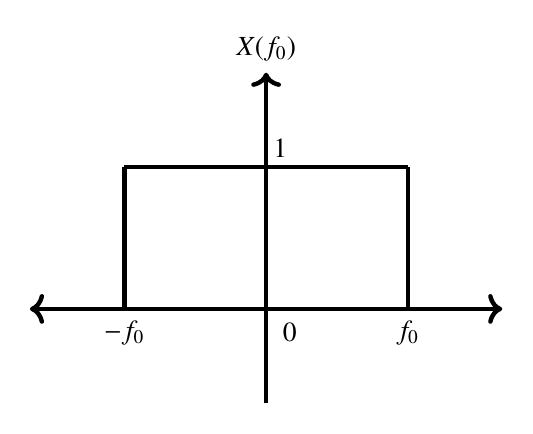
\begin{tikzpicture}[scale=0.6, ultra thick]
        \draw[->] (0,-2) -- (0,5);
        \draw (0,5.5) node {$X(f_{0}$)};
        \draw (0.5,-0.5)  node{0};
        \draw[<->]  (-5,0) -- (5,0);
        \draw  (3,3) -- (3,0);
        \draw (0.3,3.4) node{1};
        \draw (-3,3) -- (3,3);
        \draw (-3,3)--(-3,0);
        \draw (-3,-0.5) node {$-f_{0}$};

        \draw (3,-0.5) node {$f_{0}$};
    \end{tikzpicture}
\end{center}

By taking inverse Fourier transform,
\begin{align}
x\brak{t} = \frac{\sin\brak{ t}}{\pi t}
\end{align}

\begin{align}
& x\left(\frac{\pi}{2\brak{2\pi f_{0}}}\right) =\frac{2 \brak{2\pi f_{0}}}{\pi^2}
\end{align}

So, option \brak{C} and \brak{D} are wrong.

\begin{align}
x\brak{0}=\lim_{t\to 0}\frac{\sin \brak{2\pi f_{0}} t}{\pi t}=\frac{2\pi f_{0}}{\pi}
\end{align}

So, $x\brak{0} \propto f_{0} \Rightarrow$ Option \brak{B} is wrong.\\

When $f_{0}\rightarrow \infty$, $X\brak{f_{0}}$ will be a D.C signal and inverse Fourier transform of a D.C signal will be impulse signal\\[3ex]
So, option \brak{A} is correct
\begin{figure}[ht]
    \centering
    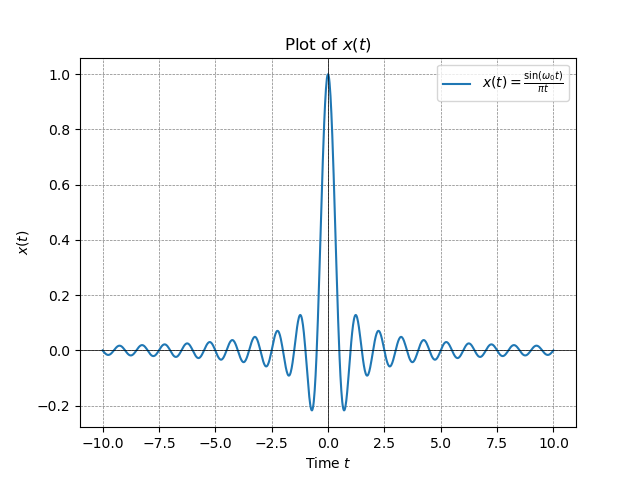
\includegraphics[width=1\columnwidth]{2023/EE/18/figs/main.png}
    \caption{plot of X\brak{t}}
    \label{fig:EE18.1}
\end{figure}


\newpage

\item \textbf{Question}:The initial value problem
$\frac{dy}{dt}+2y=0, y(0)=1 $
is solved numerically using the forward Euler's method with a constant and positive time step of $\delta $.\\
Let $y_n$ represent the numerical solution obtained after $n$ steps. The condition $\abs{y_{n+1}} \leq \abs{y_n}$is satisfied if and only if $\delta$ does not exceed \\
\hfill{(GATE ME 2023)}\\
\solution 
\input{2023/ME/50/problem3.tex}
\newpage

\item In the context of signals and systems, determine the phase cross-over frequency of the open-loop transfer function
\[
G(s) = \frac{k \cdot s \cdot (1+sT_1) \cdot (1+sT_2)}{s}
\]
with positive constants $k, T_1, T_2$ are positive constants.The phase crossover fequency,in rad/s,is
\begin{enumerate}
  \item[(a)] $\frac{1}{\sqrt{T_1 T_2}}$
  \item[(b)] $\frac{1}{T_1 T_2}$
  \item[(c)] $\frac{1}{T_1\sqrt{T_2}}$
  \item[(d)] $\frac{1}{\sqrt{T_2}T_1}$
\end{enumerate}
\hfill{(GATE EC 2023)}\\
\solution
\iffalse
\let\negmedspace\undefined
\let\negthickspace\undefined
\documentclass[journal,12pt,twocolumn]{IEEEtran}
\usepackage{cite}
\usepackage{amsmath,amssymb,amsfonts,amsthm}
\usepackage{algorithmic}
\usepackage{graphicx}
\usepackage{textcomp}
\usepackage{xcolor}
\usepackage{txfonts}
\usepackage{listings}
\usepackage{enumitem}
\usepackage{mathtools}
\usepackage{gensymb}
\usepackage{comment}
\usepackage[breaklinks=true]{hyperref}
\usepackage{tkz-euclide} 
\usepackage{listings}
\usepackage{gvv}                                        
\def\inputGnumericTable{}                                 
\usepackage[latin1]{inputenc}                                
\usepackage{color}                                            
\usepackage{array}                                            
\usepackage{longtable}                                       
\usepackage{calc}                                             
\usepackage{multirow}                                         
\usepackage{hhline}                                           
\usepackage{ifthen}                                           
\usepackage{lscape}


\newtheorem{theorem}{Theorem}[section]
\newtheorem{problem}{Problem}
\newtheorem{proposition}{Proposition}[section]
\newtheorem{lemma}{Lemma}[section]
\newtheorem{corollary}[theorem]{Corollary}
\newtheorem{example}{Example}[section]
\newtheorem{definition}[problem]{Definition}
\newcommand{\BEQA}{\begin{eqnarray}}
\newcommand{\EEQA}{\end{eqnarray}}
\newcommand{\define}{\stackrel{\triangle}{=}}
\theoremstyle{remark}
\newtheorem{rem}{Remark}
\begin{document}
\parindent 0px
\bibliographystyle{IEEEtran}

\title{Gate EE - 18}
\author{EE23BTECH11216 - P.kalyan$^{}$% <-this % stops a space
}
\maketitle
\newpage
\bigskip

\renewcommand{\thefigure}{\theenumi}
\renewcommand{\thetable}{\theenumi}
\section*{Question}
The Fourier transform x$\brak{\omega}$ of  the signal x\brak{t} is given by

\[
X(\omega) = 
\begin{cases} 
1, \text{for } |\omega| < \omega_0 \\
0, \text{for } |\omega| > \omega_0 
\end{cases}
\]

\text{(A) } x\brak{t} \text{ tends to be an impulse as } $W_0$ $\rightarrow \infty$.

\text{(B) } x\brak{0} \text{ decreases as } $W_0$ \text{ increases.}

\text{(C) At } t = $\frac{\pi}{2W_0}$, \quad x\brak{t} = -$\frac{1}{\pi}$.

\text{(D) At } t = $\frac{\pi}{2W_0}$, \quad x\brak{t} = $\frac{1}{\pi}$. \hfill\brak{\text{GATE EE 2023}}


 \fi

\begin{center}
    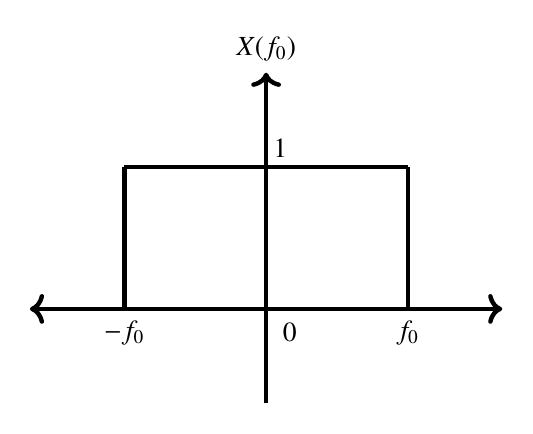
\begin{tikzpicture}[scale=0.6, ultra thick]
        \draw[->] (0,-2) -- (0,5);
        \draw (0,5.5) node {$X(f_{0}$)};
        \draw (0.5,-0.5)  node{0};
        \draw[<->]  (-5,0) -- (5,0);
        \draw  (3,3) -- (3,0);
        \draw (0.3,3.4) node{1};
        \draw (-3,3) -- (3,3);
        \draw (-3,3)--(-3,0);
        \draw (-3,-0.5) node {$-f_{0}$};

        \draw (3,-0.5) node {$f_{0}$};
    \end{tikzpicture}
\end{center}

By taking inverse Fourier transform,
\begin{align}
x\brak{t} = \frac{\sin\brak{ t}}{\pi t}
\end{align}

\begin{align}
& x\left(\frac{\pi}{2\brak{2\pi f_{0}}}\right) =\frac{2 \brak{2\pi f_{0}}}{\pi^2}
\end{align}

So, option \brak{C} and \brak{D} are wrong.

\begin{align}
x\brak{0}=\lim_{t\to 0}\frac{\sin \brak{2\pi f_{0}} t}{\pi t}=\frac{2\pi f_{0}}{\pi}
\end{align}

So, $x\brak{0} \propto f_{0} \Rightarrow$ Option \brak{B} is wrong.\\

When $f_{0}\rightarrow \infty$, $X\brak{f_{0}}$ will be a D.C signal and inverse Fourier transform of a D.C signal will be impulse signal\\[3ex]
So, option \brak{A} is correct
\begin{figure}[ht]
    \centering
    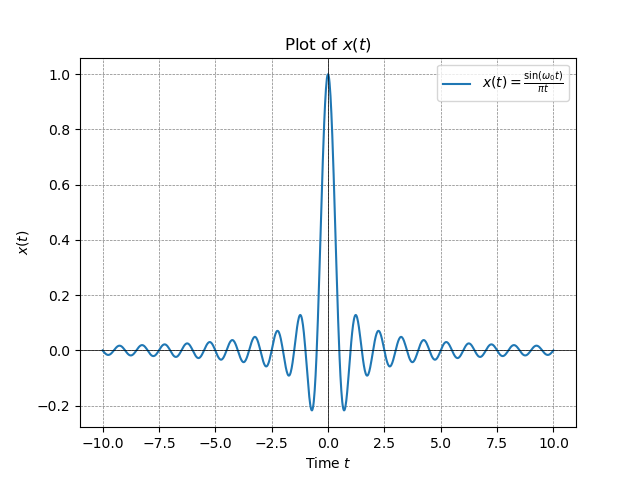
\includegraphics[width=1\columnwidth]{2023/EE/18/figs/main.png}
    \caption{plot of X\brak{t}}
    \label{fig:EE18.1}
\end{figure}


\newpage

\item Which one of the options given is the inverse Laplace transform of $\frac{1}{s^3-s}$?\\
$u(t)$ denotes the unit-step function.
\begin{enumerate}[label=(\Alph*)]
\item $\left(-1+\frac{1}{2}e^{-t}+\frac{1}{2}e^t\right)u(t)$\\
\item $\left(\frac{1}{3}e^{-t}-e^t\right)u(t)$\\
\item $\left(-1+\frac{1}{2}e^{-(t-1)}+\frac{1}{2}e^{(t-1)}\right)u(t-1)$\\
\item $\left(-1-\frac{1}{2}e^{-(t-1)}-\frac{1}{2}e^{(t-1)}\right)u(t-1)$\\
\end{enumerate}
\hfill(GATE ME 2023)\\
\solution
\iffalse
\let\negmedspace\undefined
\let\negthickspace\undefined
\documentclass[journal,12pt,twocolumn]{IEEEtran}
\usepackage{cite}
\usepackage{amsmath,amssymb,amsfonts,amsthm}
\usepackage{algorithmic}
\usepackage{graphicx}
\usepackage{textcomp}
\usepackage{xcolor}
\usepackage{txfonts}
\usepackage{listings}
\usepackage{enumitem}
\usepackage{mathtools}
\usepackage{gensymb}
\usepackage{comment}
\usepackage[breaklinks=true]{adjustbox}
\usepackage{tkz-euclide} 
\usepackage{listings}
\usepackage{gvv}                                        
\def\inputGnumericTable{}                                 
\usepackage[latin1]{inputenc}                                
\usepackage{color}                                            
\usepackage{array}                                            
\usepackage{longtable}                                       
\usepackage{calc}                                             
\usepackage{multirow}                                         
\usepackage{hhline}                                           
\usepackage{ifthen}                                           
\usepackage{lscape}

\newtheorem{theorem}{Theorem}[section]
\newtheorem{problem}{Problem}
\newtheorem{proposition}{Proposition}[section]
\newtheorem{lemma}{Lemma}[section]
\newtheorem{corollary}[theorem]{Corollary}
\newtheorem{example}{Example}[section]
\newtheorem{definition}[problem]{Definition}
\newcommand{\BEQA}{\begin{eqnarray}}
\newcommand{\EEQA}{\end{eqnarray}}
\newcommand{\define}{\stackrel{\triangle}{=}}
\theoremstyle{remark}
\newtheorem{rem}{Remark}

\begin{document}
\bibliographystyle{IEEEtran}

\vspace{3cm}

\title{}
\author{EE23BTECH11024 - G.Karthik Yadav$^{*}$
}
\maketitle
\newpage
\bigskip

\section*{GATE 2023 EC 41}
\noindent 1. \hspace{2pt} A Closed loop systen is shown in the figure where $k>0$ and $\alpha>0$ .\\
The Steady State error due to a ramp input $\brak{R\brak{s} = \alpha s^{-2}}$ is given by \hfill{(GATE 2023 EC 41)}

\begin{figure}[ht]
\centering
    \includegraphics[width=1.0\linewidth]{2023/EC/41/figs/question.png}
    \label{fig: 23.EC.41.24.1}
\end{figure}

\begin{enumerate}
\item $\frac{2\alpha}{k}$
\item $\frac{\alpha}{k}$
\item $\frac{\alpha}{2k}$
\item $\frac{\alpha}{4k}$
\end{enumerate}

\solution\\
\fi
\begin{table}[ht]
\setlength{\arrayrulewidth}{0.3mm}
\setlength{\tabcolsep}{15pt}
\renewcommand{\arraystretch}{1.5}



\begin{tabular}{ |p{1cm}|p{3cm}|p{1cm}| }
\hline
Symbol & Parameters & Value\\
\hline
$R\brak{s}$ & Laplace transform Ramp input signal r\brak{t} &  $\alpha s^{-2}$\\
\hline
$G\brak{s}$ & Open Loop transfer function &  $ \frac{Y\brak{s}}{E\brak{s}} = \frac{k}{s\brak{s+2}}$\\
\hline
$Y\brak{s}$ & Laplace transform of the output signal y\brak{t}  &  ? \\
\hline
$E\brak{s}$ & Laplace transform of the error signal e\brak{t} & R\brak{s} - Y\brak{s}\\
\hline
$E\brak{s}$ & Laplace transform of the error signal e\brak{t} & R\brak{s} - Y\brak{s}\\   
\hline
$e_s$ & Steady State Error &  ? \\
\hline
%$x(l)$ & Last($l^{th}$) term of series & 350\\
%$x(0)$ & Starting ($0^{th}$) term of series & 17 %\\
%\hline
%d & Common difference of AP & 9\\
%\hline
\end{tabular}
\caption{Parameters}






\end{table}
\bigskip
from table  Open loop transfer function $G\brak{s}$\\
\begin{align}
	G\brak{s} &= \frac{Y\brak{s}}{E\brak{s}} \label{24.2023.EC.41.1} \\
        &= \frac{Y\brak{s}}{R\brak{s} - Y\brak{s}} \\
        Y\brak{s} &= \frac{R\brak{s}G\brak{s}}{1 + G\brak{s}} \label{24.2023.EC.41.2}
\end{align}

from eq \ref{24.2023.EC.41.1} and eq \eqref{24.2023.EC.41.2}

\begin{align}
        G\brak{s} &= \frac{k}{s\brak{s +2}}  \label{24.2023.EC.41.3} \\ 
        Y\brak{s} &= \frac{\alpha k s^{-2}}{k + s\brak{s+2}} \label{24.2023.EC.41.4} \\
        E\brak{s} &= R\brak{s} - Y\brak{s}  \label{24.2023.EC.41.5} \\ 
        E\brak{s} &= \frac{\alpha \brak{s+2}}{s\brak{k + s\brak{s+2}}}
\end{align}

By Taking Inverse Laplace Transform of eq \eqref{24.2023.EC.41.3} and eq\eqref{24.2023.EC.41.4}

\begin{align}
    g\brak{t} &= \frac{k\brak{1 - e^{-2t}}}{2} u\brak{t} \\
        y\brak{t} &= \alpha t u\brak{t}- \frac{2\alpha}{k}u\brak{t} \\
        \notag &+\frac{\alpha}{2k\sqrt{1-k}} \biggl(2\sqrt{1-k}e^{\sqrt{1-k}t-1}\\ 
        \notag &+ 2\sqrt{1-k}e^{-\sqrt{1-k}t-1} \\
        \notag &+ \brak{2-k}e^{\sqrt{1-k}t-1} - \brak{2-k}e^{-\sqrt{1-k}t-1} \biggr) u\brak{t}
\end{align}

\begin{align}
        e\brak{t} &= r\brak{t} - y\brak{t} \\
        &= \alpha t u\brak{t} - y\brak{t} \\
        e\brak{t} &= \frac{2\alpha}{k}u\brak{t} \\
        \notag &-\frac{\alpha}{2k\sqrt{1-k}} \biggl(2\sqrt{1-k}e^{\sqrt{1-k}t-1}\\ 
        \notag &+ 2\sqrt{1-k}e^{-\sqrt{1-k}t-1} \\
        \notag &+ \brak{2-k}e^{\sqrt{1-k}t-1} - \brak{2-k}e^{-\sqrt{1-k}t-1} \biggr) u\brak{t}
\end{align}
	

\begin{align}
    e_s &= \displaystyle\lim_{s\to 0}s E\brak{s} \\
    &= \displaystyle\lim_{s\to 0} s \frac{R\brak{s}}{1 + G\brak{s}} \\
    &= \displaystyle\lim_{s\to 0} \frac{\alpha \brak{s+2}}{s\brak{s+2} + k} \\
    e_s &= \frac{2\alpha}{k}
\end{align}



\newpage

\item The state equation of a second order system is \\
$ \dot{{x}}(t) = A{x}(t)$, \quad ${x}(0)$ is the initial condition. \\
Suppose $\lambda_1$ and $\lambda_2$ are two distinct eigenvalues of $A$, and $\nu_1$ and $\nu_2$ are the corresponding eigenvectors. For constants $\alpha_1$ and $\alpha_2$, the solution, ${x}(t)$, of the state equation is \\
\begin{enumerate}[label=(\Alph*)]
\item $\sum_{i=1}^{2} \alpha_ie^{\lambda_it}\bf{\nu}_i$
\item $\sum_{i=1}^{2} \alpha_ie^{2\lambda_it}\bf{\nu}_i$
\item $\sum_{i=1}^{2} \alpha_ie^{3\lambda_it}\bf{\nu}_i$
\item $\sum_{i=1}^{2} \alpha_ie^{4\lambda_it}\bf{\nu}_i$
\end{enumerate}
\hfill{GATE EC 2023}\\
\solution
\iffalse
\let\negmedspace\undefined
\let\negthickspace\undefined
\documentclass[journal,12pt,twocolumn]{IEEEtran}
\usepackage{cite}
\usepackage{amsmath,amssymb,amsfonts,amsthm}
\usepackage{algorithmic}
\usepackage{graphicx}
\usepackage{textcomp}
\usepackage{xcolor}
\usepackage{txfonts}
\usepackage{listings}
\usepackage{enumitem}
\usepackage{mathtools}
\usepackage{gensymb}
\usepackage{comment}
\usepackage[breaklinks=true]{adjustbox}
\usepackage{tkz-euclide} 
\usepackage{listings}
\usepackage{gvv}                                        
\def\inputGnumericTable{}                                 
\usepackage[latin1]{inputenc}                                
\usepackage{color}                                            
\usepackage{array}                                            
\usepackage{longtable}                                       
\usepackage{calc}                                             
\usepackage{multirow}                                         
\usepackage{hhline}                                           
\usepackage{ifthen}                                           
\usepackage{lscape}

\newtheorem{theorem}{Theorem}[section]
\newtheorem{problem}{Problem}
\newtheorem{proposition}{Proposition}[section]
\newtheorem{lemma}{Lemma}[section]
\newtheorem{corollary}[theorem]{Corollary}
\newtheorem{example}{Example}[section]
\newtheorem{definition}[problem]{Definition}
\newcommand{\BEQA}{\begin{eqnarray}}
\newcommand{\EEQA}{\end{eqnarray}}
\newcommand{\define}{\stackrel{\triangle}{=}}
\theoremstyle{remark}
\newtheorem{rem}{Remark}

\begin{document}
\bibliographystyle{IEEEtran}

\vspace{3cm}

\title{}
\author{EE23BTECH11024 - G.Karthik Yadav$^{*}$
}
\maketitle
\newpage
\bigskip

\section*{GATE 2023 EC 41}
\noindent 1. \hspace{2pt} A Closed loop systen is shown in the figure where $k>0$ and $\alpha>0$ .\\
The Steady State error due to a ramp input $\brak{R\brak{s} = \alpha s^{-2}}$ is given by \hfill{(GATE 2023 EC 41)}

\begin{figure}[ht]
\centering
    \includegraphics[width=1.0\linewidth]{2023/EC/41/figs/question.png}
    \label{fig: 23.EC.41.24.1}
\end{figure}

\begin{enumerate}
\item $\frac{2\alpha}{k}$
\item $\frac{\alpha}{k}$
\item $\frac{\alpha}{2k}$
\item $\frac{\alpha}{4k}$
\end{enumerate}

\solution\\
\fi
\begin{table}[ht]
\setlength{\arrayrulewidth}{0.3mm}
\setlength{\tabcolsep}{15pt}
\renewcommand{\arraystretch}{1.5}



\begin{tabular}{ |p{1cm}|p{3cm}|p{1cm}| }
\hline
Symbol & Parameters & Value\\
\hline
$R\brak{s}$ & Laplace transform Ramp input signal r\brak{t} &  $\alpha s^{-2}$\\
\hline
$G\brak{s}$ & Open Loop transfer function &  $ \frac{Y\brak{s}}{E\brak{s}} = \frac{k}{s\brak{s+2}}$\\
\hline
$Y\brak{s}$ & Laplace transform of the output signal y\brak{t}  &  ? \\
\hline
$E\brak{s}$ & Laplace transform of the error signal e\brak{t} & R\brak{s} - Y\brak{s}\\
\hline
$E\brak{s}$ & Laplace transform of the error signal e\brak{t} & R\brak{s} - Y\brak{s}\\   
\hline
$e_s$ & Steady State Error &  ? \\
\hline
%$x(l)$ & Last($l^{th}$) term of series & 350\\
%$x(0)$ & Starting ($0^{th}$) term of series & 17 %\\
%\hline
%d & Common difference of AP & 9\\
%\hline
\end{tabular}
\caption{Parameters}






\end{table}
\bigskip
from table  Open loop transfer function $G\brak{s}$\\
\begin{align}
	G\brak{s} &= \frac{Y\brak{s}}{E\brak{s}} \label{24.2023.EC.41.1} \\
        &= \frac{Y\brak{s}}{R\brak{s} - Y\brak{s}} \\
        Y\brak{s} &= \frac{R\brak{s}G\brak{s}}{1 + G\brak{s}} \label{24.2023.EC.41.2}
\end{align}

from eq \ref{24.2023.EC.41.1} and eq \eqref{24.2023.EC.41.2}

\begin{align}
        G\brak{s} &= \frac{k}{s\brak{s +2}}  \label{24.2023.EC.41.3} \\ 
        Y\brak{s} &= \frac{\alpha k s^{-2}}{k + s\brak{s+2}} \label{24.2023.EC.41.4} \\
        E\brak{s} &= R\brak{s} - Y\brak{s}  \label{24.2023.EC.41.5} \\ 
        E\brak{s} &= \frac{\alpha \brak{s+2}}{s\brak{k + s\brak{s+2}}}
\end{align}

By Taking Inverse Laplace Transform of eq \eqref{24.2023.EC.41.3} and eq\eqref{24.2023.EC.41.4}

\begin{align}
    g\brak{t} &= \frac{k\brak{1 - e^{-2t}}}{2} u\brak{t} \\
        y\brak{t} &= \alpha t u\brak{t}- \frac{2\alpha}{k}u\brak{t} \\
        \notag &+\frac{\alpha}{2k\sqrt{1-k}} \biggl(2\sqrt{1-k}e^{\sqrt{1-k}t-1}\\ 
        \notag &+ 2\sqrt{1-k}e^{-\sqrt{1-k}t-1} \\
        \notag &+ \brak{2-k}e^{\sqrt{1-k}t-1} - \brak{2-k}e^{-\sqrt{1-k}t-1} \biggr) u\brak{t}
\end{align}

\begin{align}
        e\brak{t} &= r\brak{t} - y\brak{t} \\
        &= \alpha t u\brak{t} - y\brak{t} \\
        e\brak{t} &= \frac{2\alpha}{k}u\brak{t} \\
        \notag &-\frac{\alpha}{2k\sqrt{1-k}} \biggl(2\sqrt{1-k}e^{\sqrt{1-k}t-1}\\ 
        \notag &+ 2\sqrt{1-k}e^{-\sqrt{1-k}t-1} \\
        \notag &+ \brak{2-k}e^{\sqrt{1-k}t-1} - \brak{2-k}e^{-\sqrt{1-k}t-1} \biggr) u\brak{t}
\end{align}
	

\begin{align}
    e_s &= \displaystyle\lim_{s\to 0}s E\brak{s} \\
    &= \displaystyle\lim_{s\to 0} s \frac{R\brak{s}}{1 + G\brak{s}} \\
    &= \displaystyle\lim_{s\to 0} \frac{\alpha \brak{s+2}}{s\brak{s+2} + k} \\
    e_s &= \frac{2\alpha}{k}
\end{align}



\newpage

\item The continuous time signal $x\brak{t}$ is described by:
\begin{align}
x\brak{t}=
    \begin{cases}
        1, & \text{if } 0\: {\displaystyle \leq }\:t\:{\displaystyle \leq }\:1\\
        0, & \text{elsewhere}
    \end{cases} 
\end{align}
If $y\brak{t}$ represents $x\brak{t}$ convolved with itself, which of the following options is/are TRUE?
\begin{enumerate}[label = (\Alph*)]
    \item $y\brak{t}$ = 0 for all $t<0$ \label{gate.bm.49.a}\\
    \item $y\brak{t}$ = 0 for all $t>1$ \label{gate.bm.49.b}\\
    \item $y\brak{t}$ = 0 for all $t>3$ \label{gate.bm.49.c}\\
    \item $\int_{0.1}^{0.75} \frac{dy\brak{t}}{dt}\: \text{dt} \neq 0$ \label{gate.bm.49.d}
\end{enumerate} \hfill{GATE 2023 BM- Q 49}\\
\input{2023/BM/49/gate.bm.49.tex}
\newpage

\item For the signals x\brak{t} and y\brak{t} shown in the figure, $z\brak{t}=x\brak{t}*y\brak{t}$ is maximum at $t=T_1$. Then $T_1$ in seconds is .......... \brak{\text{Round off to the nearest integer}}\\
\input{2023/EE/31/figs/codes/plot1.tex}
\input{2023/EE/31/figs/codes/plot2.tex}
\hfill (GATE EE 2023 Q 31)
\solution
\iffalse
\let\negmedspace\undefined
\let\negthickspace\undefined
\documentclass[journal,12pt,twocolumn]{IEEEtran}
\usepackage{cite}
\usepackage{amsmath,amssymb,amsfonts,amsthm}
\usepackage{algorithmic}
\usepackage{graphicx}
\usepackage{textcomp}
\usepackage{xcolor}
\usepackage{txfonts}
\usepackage{listings}
\usepackage{enumitem}
\usepackage{mathtools}
\usepackage{gensymb}
\usepackage{comment}
\usepackage[breaklinks=true]{hyperref}
\usepackage{tkz-euclide} 
\usepackage{listings}
\usepackage{gvv}                                        
\def\inputGnumericTable{}                                 
\usepackage[latin1]{inputenc}                                
\usepackage{color}                                            
\usepackage{array}                                            
\usepackage{longtable}                                       
\usepackage{calc}                                             
\usepackage{multirow}                                         
\usepackage{hhline}                                           
\usepackage{ifthen}                                           
\usepackage{lscape}


\newtheorem{theorem}{Theorem}[section]
\newtheorem{problem}{Problem}
\newtheorem{proposition}{Proposition}[section]
\newtheorem{lemma}{Lemma}[section]
\newtheorem{corollary}[theorem]{Corollary}
\newtheorem{example}{Example}[section]
\newtheorem{definition}[problem]{Definition}
\newcommand{\BEQA}{\begin{eqnarray}}
\newcommand{\EEQA}{\end{eqnarray}}
\newcommand{\define}{\stackrel{\triangle}{=}}
\theoremstyle{remark}
\newtheorem{rem}{Remark}
\begin{document}
\parindent 0px
\bibliographystyle{IEEEtran}

\title{Gate EE - 18}
\author{EE23BTECH11216 - P.kalyan$^{}$% <-this % stops a space
}
\maketitle
\newpage
\bigskip

\renewcommand{\thefigure}{\theenumi}
\renewcommand{\thetable}{\theenumi}
\section*{Question}
The Fourier transform x$\brak{\omega}$ of  the signal x\brak{t} is given by

\[
X(\omega) = 
\begin{cases} 
1, \text{for } |\omega| < \omega_0 \\
0, \text{for } |\omega| > \omega_0 
\end{cases}
\]

\text{(A) } x\brak{t} \text{ tends to be an impulse as } $W_0$ $\rightarrow \infty$.

\text{(B) } x\brak{0} \text{ decreases as } $W_0$ \text{ increases.}

\text{(C) At } t = $\frac{\pi}{2W_0}$, \quad x\brak{t} = -$\frac{1}{\pi}$.

\text{(D) At } t = $\frac{\pi}{2W_0}$, \quad x\brak{t} = $\frac{1}{\pi}$. \hfill\brak{\text{GATE EE 2023}}


 \fi

\begin{center}
    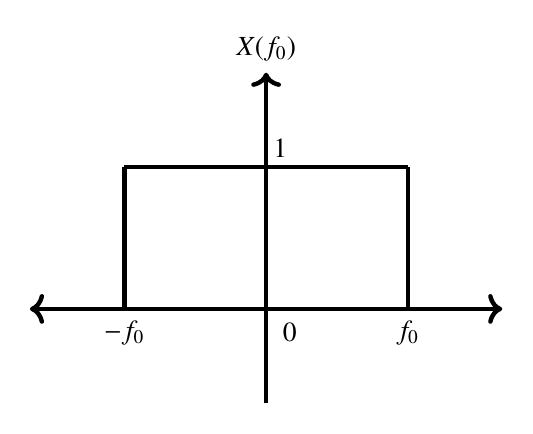
\begin{tikzpicture}[scale=0.6, ultra thick]
        \draw[->] (0,-2) -- (0,5);
        \draw (0,5.5) node {$X(f_{0}$)};
        \draw (0.5,-0.5)  node{0};
        \draw[<->]  (-5,0) -- (5,0);
        \draw  (3,3) -- (3,0);
        \draw (0.3,3.4) node{1};
        \draw (-3,3) -- (3,3);
        \draw (-3,3)--(-3,0);
        \draw (-3,-0.5) node {$-f_{0}$};

        \draw (3,-0.5) node {$f_{0}$};
    \end{tikzpicture}
\end{center}

By taking inverse Fourier transform,
\begin{align}
x\brak{t} = \frac{\sin\brak{ t}}{\pi t}
\end{align}

\begin{align}
& x\left(\frac{\pi}{2\brak{2\pi f_{0}}}\right) =\frac{2 \brak{2\pi f_{0}}}{\pi^2}
\end{align}

So, option \brak{C} and \brak{D} are wrong.

\begin{align}
x\brak{0}=\lim_{t\to 0}\frac{\sin \brak{2\pi f_{0}} t}{\pi t}=\frac{2\pi f_{0}}{\pi}
\end{align}

So, $x\brak{0} \propto f_{0} \Rightarrow$ Option \brak{B} is wrong.\\

When $f_{0}\rightarrow \infty$, $X\brak{f_{0}}$ will be a D.C signal and inverse Fourier transform of a D.C signal will be impulse signal\\[3ex]
So, option \brak{A} is correct
\begin{figure}[ht]
    \centering
    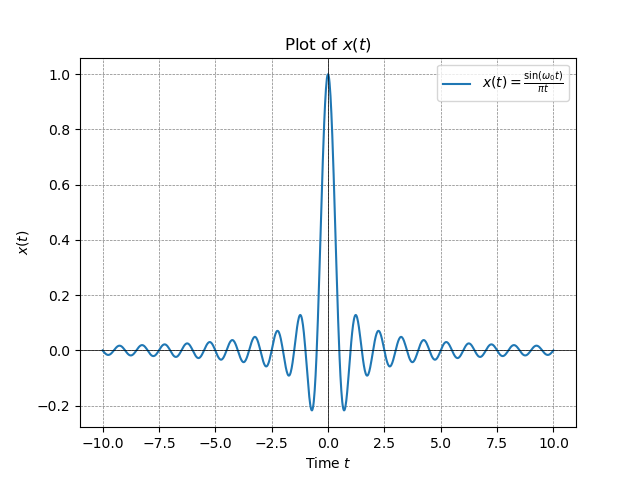
\includegraphics[width=1\columnwidth]{2023/EE/18/figs/main.png}
    \caption{plot of X\brak{t}}
    \label{fig:EE18.1}
\end{figure}


\newpage

\end{enumerate}
